\section{Systementwurf}
\textcolor{red}{Lorem ipsum dolor sit amet, consetetur sadipscing elitr, sed diam nonumy eirmod tempor invidunt ut labore et dolore magna aliquyam erat, sed diam voluptua. Lorem ipsum dolor sit amet, consetetur sadipscing elitr, sed diam nonumy eirmod tempor invidunt ut labore et dolore magna aliquyam erat, sed diam voluptua. Lorem ipsum dolor sit amet, consetetur sadipscing elitr, sed diam nonumy eirmod tempor invidunt ut labore et dolore magna aliquyam erat, sed diam voluptua. Lorem ipsum dolor sit amet, consetetur sadipscing elitr, sed diam nonumy eirmod tempor invidunt ut labore et dolore magna aliquyam erat, sed diam voluptua.}

\subsection{Vorgehensweise Anforderungserhebung}
Die Anforderungen für ein zu konzipierende System wurden vor dem Hintergrund der Evaluation des Geschäftsprozesses erhoben. Außerdem wurde bei der Erfassung der Anforderung darauf geachtet, das der Prototyp beim Praxispartner als Unterstützung für zukünftige Innovationsfragen herangezogen werden kann. Wie von \citet{Dick2017, HullElizabeth2011} beschrieben, kann das Prototyping selbst bereits als Anforderungsanalyse angesehen werden, jedoch wurde für die prototypische Implementierung des Systementwurfs eine gesonderte Anforderungsanalyse durchgeführt. Ziel dieser Vorgehensweise ist eine präzise Definition und Eingrenzung der Anforderungsbeschreibung während des Konzeptions- und Implementierungsprozesses.

Im Zuge der Anforderungserhebung wurden die Anforderungen in Zusammenarbeit mit dem Praxispartner entwickelt. Die Anforderungen wurden dabei in textueller Form nach einem festen Muster in Anlehnung an \citet{PohlKlaus2015} definiert. Ergänzt wurden die textuellen Anforderungen um Prozessdiagramme und Mockups der Nutzeroberflächen. Der Fokus des konzipierten System liegt dabei allerdings auf eigentlichen Blockchain Netzwerk und weniger auf der Benutzungsoberfläche.

Die Anforderungen wurden untergliedert in funktionale Anforderungen, Rahmenbedingungen und Qualitätsanforderungen. Ebenso wurden die Anforderungen hierarchisch strukturiert und um eine Quelle ergänzt nach \citet{Koelsch2016}. Dies soll die Nachverfolgbarkeit der Anforderungen während der Evaluation unterstützen.

\subsection{Das Ziel: Chargenrückverfolgung innerhalb der Fleischwarenindustrie} \label{goal-description}
Das System soll unter experimentellen, abstrahierten Bedingungen die Chargenrückverfolgung von Schweinen innerhalb der Produktions- und Wertschöpfungskette realisieren. Dafür muss das System den Prozess vom Erzeuger bis zum Groß- und Einzelhandel unterstützen. Konkret sollen Erzeuger neue Tiere im Blockchain Netzwerk registrieren und einer Charge zuordnen können. Bereits registrierte Tiere sollen zur Weiterverarbeitung freigegeben werden können und ein Eigentumswechsel muss durch das System abbildbar sein. Die Gesamtheit der Transaktionen zwischen den Teilnehmern der Wertschöpfungskette kann als Graph angesehen werden. Anhand dieses Graphen soll eine Rückverfolgbarkeit einer Charge gewährleistet werden. Über eine Benutzungsoberfläche sollen die Teilnehmer jederzeit in der Lage sein den Graphen einsehen zu können. Für die technische Umsetzung des System spielt die Benutzungsoberfläche jedoch eine nachgelagerte Priorität. Hauptaugenmerk des Systementwurfs liegt auf dem technologischen Aufbau des Blockchain Netzwerk und den Schnittstellen für etwaige Drittsysteme zur automatischen Erfassung von Tieren. Eine automatische Erfassung von neuen Tieren kann beispielsweise über \ac{iot}-Sensoren in Schlachthaken erfolgen. Ebenso würde sich ein Eigentumswechsel, wenn Tiere vom Erzeuger an den Schlachthof verkauft werden, über \acs{rfid}-Chips und entsprechende Lesegeräte, welche per Schnittstelle mit dem Blockchain Netzwerk verbunden sind, abwickeln lassen \citep{Dorri2017, Samaniego2016}.

\subsection{Die Wertschöpfungskette im Detail}
Nachfolgend soll eine kurze Erläuterung der in Kapitel \ref{goal-description} erwähnten Wertschöpfungskette dazu dienen, die Daten- und Warenströme zwischen den Teilnehmern klar zu trennen und die für diesen Systementwurf wichtigen Informationen herauszuarbeiten. Da eine Chargenrückverfolgung nur gewährleistet werden kann, wenn in den vorgelagerten Prozessen die nötigen Informationen in einem System bereitgestellt wurden, soll auf die Teilschritte vom Erzeuger zum Endverbraucher eingegangen werden.

Die Fleischwirtschaft hat in den letzten Jahren einen Strukturwandel vollzogen, welcher auch Auswirkungen auf die eigentliche Tätigkeit sowie die Lieferanten- und Abnehmerbeziehungen zwischen den Unternehmen hat \citep{Nolte2006}. Als eine der zentralen Ursachen für den Strukturwandel wird die Konzentrierung der Schlachtunternehmen gezählt. Inzwischen werden deutlich mehr als 50\% aller Schweine in Deutschland von drei Unternehmen geschlachtet - Tönnies, Vion und Westfleisch. Unter Beachtung anderer Wirtschaftszweige wie beispielsweise der Geflügelschlachtung, die noch wesentlich stärker konzentriert ist, und dem Hintergrund das in Ländern wie Dänemark die Schlachtung nur noch von zwei Unternehmen durchgeführt wird, wird deutlich das der Konzentrationsprozess in Deutschland auf der Schlachtstufe noch nicht abgeschlossen ist. Im Gegensatz dazu ist der Viehandel und die Landwirtschaft weniger stark konzentriert, weshalb sie sich in einer schwachen Verhandlungsposition befinden. Um dieser schwachen Verhandlungsposition entgegenzuwirken sind Unternehmen des Viehandels dazu gezwungen immer größere Mengen an Schlachttieren zu einer Charge zu bündeln. Ebenfalls sind zahlreiche unternehmensübergreifende Kooperationen im Viehandel zu beobachten \citep{Voss2010}.

Vom Erzeuger bis zum Endverbraucher ist die Wertschöpfungskette in Deutschland sehr vielfältig ausgeprägt \citep{Freund1997}. Der Hauptabsatzweg für Schweinemäster läuft entweder über eine direkt Vermarktung an Schlachtbetriebe (einstufige Vermarktung) oder indirekt über den privaten Viehandel, Viehvermarktungsgenossenschaften oder Erzeugergemeinschaften (zweistufige Vermarktung). Die Schlachtstufe lässt sich daher als Flaschenhals der Wertschöpfungskette aus Sicht der Schweinemäster betrachten. Um klar bestimmen zu können welche Informationen und virtuellen Assets in dem Blockchain Netzwerk abgebildet werden müssen, werden der Waren- und Datenstrom nachfolgend einzeln betrachtet.

\subsubsection{Betrachtung des Warenstroms}

Die Wertschöpfungskette vom Erzeuger bis zum Fleischwarenproduzenten gliedert sich grob in vier Produktionsschritte, welche nachfolgend kurz beschrieben und in Abbildung \ref{fig:structure-value-chain-meat-industry-numbered} schematisch dargestellt werden. Dabei sind sieben Parteien direkt in den Gesamtprozess bis zum Verbraucher involviert und eine achte Partei wirkt indirekt als Vermittler zwischen den anderen Parteien mit.

\begin{landscape}
    \begin{figure}
        \centering
        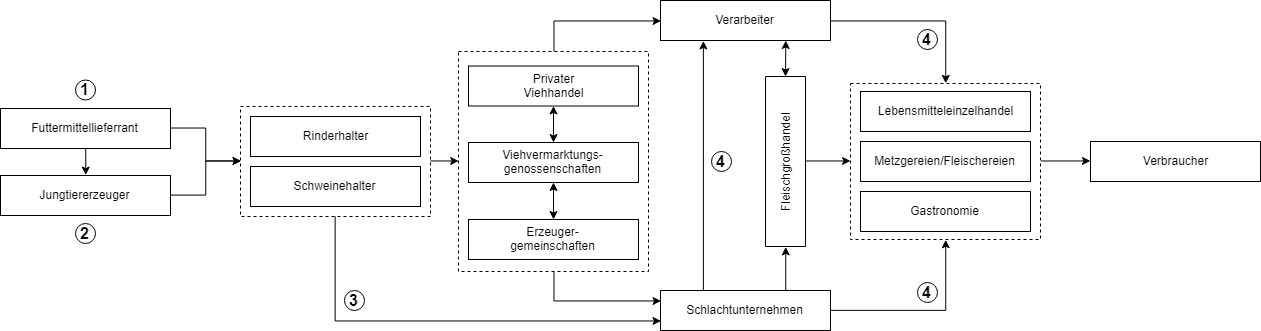
\includegraphics[width=1.0\linewidth]{pictures/structure-value-chain-meat-industry-numbered}
        \caption[Struktur der Wertschöpfungskette der Fleischwirtschaft]{Struktur der Wertschöpfungskette der Fleischwirtschaft nach \citet{Petersen2010, Voss2010, Beck2008}}
        \label{fig:structure-value-chain-meat-industry-numbered}
    \end{figure}
\end{landscape}

\noindent
Der Warenstrom beginnt mit (1) der Futtermittellieferung an die Jungtiererzeuger und Viehhalter. Jeder Betrieb wird dabei über die \ac{iln} global eindeutig identifiziert. (2) Nach der Aufzucht der Jungtiere werden diese durch Transportunternehmen zu den Viehhaltern transportiert. In den Mästbetrieben bleiben die Tiere dann bis zur Schlachtreife. (3) Im Auftrag der Schlacht- und Zerlegebetriebe werden die schlachtreifen Tiere von den Mästbetrieben angeliefert. Nach der Verarbeitung der Tiere in den Schlacht- und Zerlegebetrieben werden diese (4) an die verschiedenen Abnehmer geliefert, um letztendlich zu Produkten für den Verbraucher weiterverarbeitet zu werden. Hieraus ergibt sich, dass mindestens an den erwähnten vier Punkten der Wertschöpfungskette eine Prozessschnittstelle vom Blockchain Netzwerk bedient werden können muss.

\subsubsection{Informationswege in der Fleischindustrie}

Abbildung \ref{fig:data-stream-meat-industry} zeigt den nachfolgend beschriebenen Datenstrom zwischen den einzelnen Produktionsstufen der Fleischindustrie. \textcolor{red}{Referenz zu Anforderungen} (1) Jungtiererzeuger und Viehhalter senden jeweils eine Futtermittelbestellung an den Futtermittellieferanten. (2) Nach erfolgreicher Lieferung informiert der Futtermittellieferant den privaten Viehhandel bzw. die Viehvermarktungsgenossenschaften respektive Erzeugergemeinschaften. Die Viehhalter melden einerseits (3) die Aufnahme der Jungtiere und andererseits (4) die schlachtreife von Tieren an die Viehvermarktungsgenossenschaften zur Weitervermittlung and die Schlacht- und Zerlegebetriebe. (5) Bei der Weitervermittlung werden die Informationen über die Tiere an Schlacht- und Zerlegebetriebe übermittelt. (6) Mit dem Lieferauftrag initiiert das Schlachtunternehmen die Bestellung und den Transport der schlachtreifen Tiere. (7) Die Viehvermarktungsgenossenschaften bestätigen den Lieferauftrag mit einer elektronischen Ankündigung der Schlachtviehlieferung. Bei der Anlieferung der Tiere gleicht das Schlachtunternehmen die tatsächliche angelieferte Anzahl mit der bestellten Menge ab und meldet die Werte an die Viehvermarktungsgenossenschaften zurück. Mit dieser Wareneingangsmeldung kann die Viehvermarktungsgenossenschaft den Bestand und die aktuellen Standorte der Tiere aktualisieren. (9) Im Schlachtunternehmen werden dann weitere Informationen zu den Stammdaten der Tiere erfasst. Dazu zählen die \ac{vvvo}-Nummern der Landwirte, eine Vergabe Partie-Nummer je Lkw und eine fortlaufende Schlachtnummer. (10)Anschließend werden die Informationen wieder an die Viehvermarktungsgenossenschaft zurück gemeldet. (11) Letztendlich bedienen die Schlacht- und Zerlegebetriebe die Bestellungen der Fleischwerke, Lebensmitteleinzelhandel, Metzgereien und die Gastronomie. (12) Hier werden dann auch die letzten Stammdaten zu den Produkten erfasst und verknüpft wie beispielsweise Artikelbezeichnung, Stückzahl, Schlachtdatum und Schlacht-Nummer. (13) Mit der Zuordnung der zuverarbeitenden Fleischerzeugnisse zum Lieferschein in einem \ac{erp}-System enden die betrachteten Informationswege in der Fleischindustrie.

\begin{figure}[H]
	\centering
	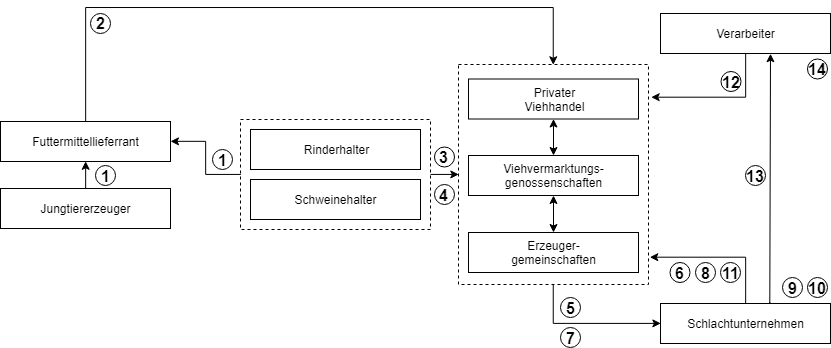
\includegraphics[width=1\linewidth]{pictures/data-stream-meat-industry-numbered}
	\caption[Datenströme innerhalb der Wertschöpfungskette]{Datenströme innerhalb der Wertschöpfungskette \textcolor{red}{QUELLE}}
	\label{fig:data-stream-meat-industry}
\end{figure}

%1 Futtermittelbestellung\\
%2 Meldung über Futtermittellieferung (DESADV optional)\\
%3 Aufnahmemeldung der Jungtiere\\
%4 Meldung schlachtreifer Schweine\\
%5 Weitervermittlung schlachtreifer Schweine an Schlachthof\\
%6 Lieferauftrag\\
%7 elektronische Ankündigung der Schlachtviehlieferung\\
%8 Wareneingangsmeldung (optional)\\
%9 Erfassung VVVO Landwirt, Vergabe Partie-Nr. je Lkw (je vom Schlachthof); Aufbringen einer fortlaufenden Schlacht-Nr. (manuell)\\
%10 Meldung Schlachtdaten\\
%11 Bestellung Schweinehälften\\
%12 u.a. Artikelbezeichnung, Stückzahl, Schlachtdatum, Schlacht-Nr., Schadenskennzeichen\\
%13 Automatische Zubuchung Schweinehälfte und Gewicht, Automatische Verknüpfung mit Lieferschein im ERP-System

\subsection{Geschäftsprozess Chargenrückverfolgung}
Die vorrangegangene Betrachtung der Waren- und Datenströme macht deutlich an welchen Schnittpunkten der Wertschöpfungskette Informationen gesammelt und zentral über die Viehvermarktungsgenossenschaften verwaltet werden. Dies ist wichtig für den Geschäftsprozess der Chargenrückverfolgung, da eine lückenlose Rückverfolgbarkeit nur dann gewährleistet ist wenn vom Erzeuger bis zum Endverbraucher alle Informationen konsistent und transparent zur Verfügung stehen. Dabei spielt es keine Rolle von welcher Seite der Wertschöpfungskette eine Rückverfolgung durchgeführt wird im Sinne des Down- und Uptracing.

Der Vergleich zwischen dem Prozess der Rückverfolgung wie er aktuell durchgeführt wird (Ist-Prozess) und wie er mit dem Einsatz eines Blockchain Systems aussehen kann (Soll-Prozess) dient dazu die funktionalen Anforderungen ableiten zu können.

\paragraph{Ist-Prozess}
Der Ist-Prozess (Abbildung \ref{fig:business-process-epc-diagramm}) durchläuft die Schritte von der Verbrauchermeldung bis zur Information der anderen Teilnehmer in der Wertschöpfungskette. Dabei wird anhand der Produktkennung und Verbrauchermeldung ermittelt zu welcher Produktcharge die Meldung gehört. Hierfür wird eine vielzahl an Software und Datenbeständen benötigt. Dazu zählt die Office Suite von Microsoft und ein ERP-System in Kombination mit einer Lieferantenmanagement- (SAP SRM) und Vertriebslösung (SAP CRM). Nach der Zuordnung der Verbrauchermeldung zur Produktcharge wird im Sinne des Uptracing die Charge bis zum Erzeuger zurückverfolgt, um zu prüfen in welchem Produktionsschritt das gemeldete Problem entstanden ist. Hierdurch können Maßnahmen zum Abstellen des Problem erarbeitet werden, die an alle Teilnehmer übermittelt werden. Die Chargeninformationen werden bereitsgestellt von einer zentralen Instanz, der Viehvermarktungsgenossenschaft. Dies bedeutet, liegen der Viehvermarktungsgenossenschaft lückenhafte bzw. manipulierte Datensätze vor besteht die Gefahr eine Rückverfolgung nicht vollständig durchführen zu können. Ebenfalls muss der Verbraucher der Viehvermarktungsgenossenschaft vertrauen für vollständig- und korrektheit der bereitgestellten Informationen. Nachdem alle Teilnehmer informiert sind ist der Prozess der Rückverfolgung abgeschlossen. Entsprechende folge Prozesse für einen eventuellen Rückruf von Produkten werden beim Abschluss der Rückverfolgung teils automatisch teils manuell ausgelöst.

\begin{figure}[H]
	\centering
	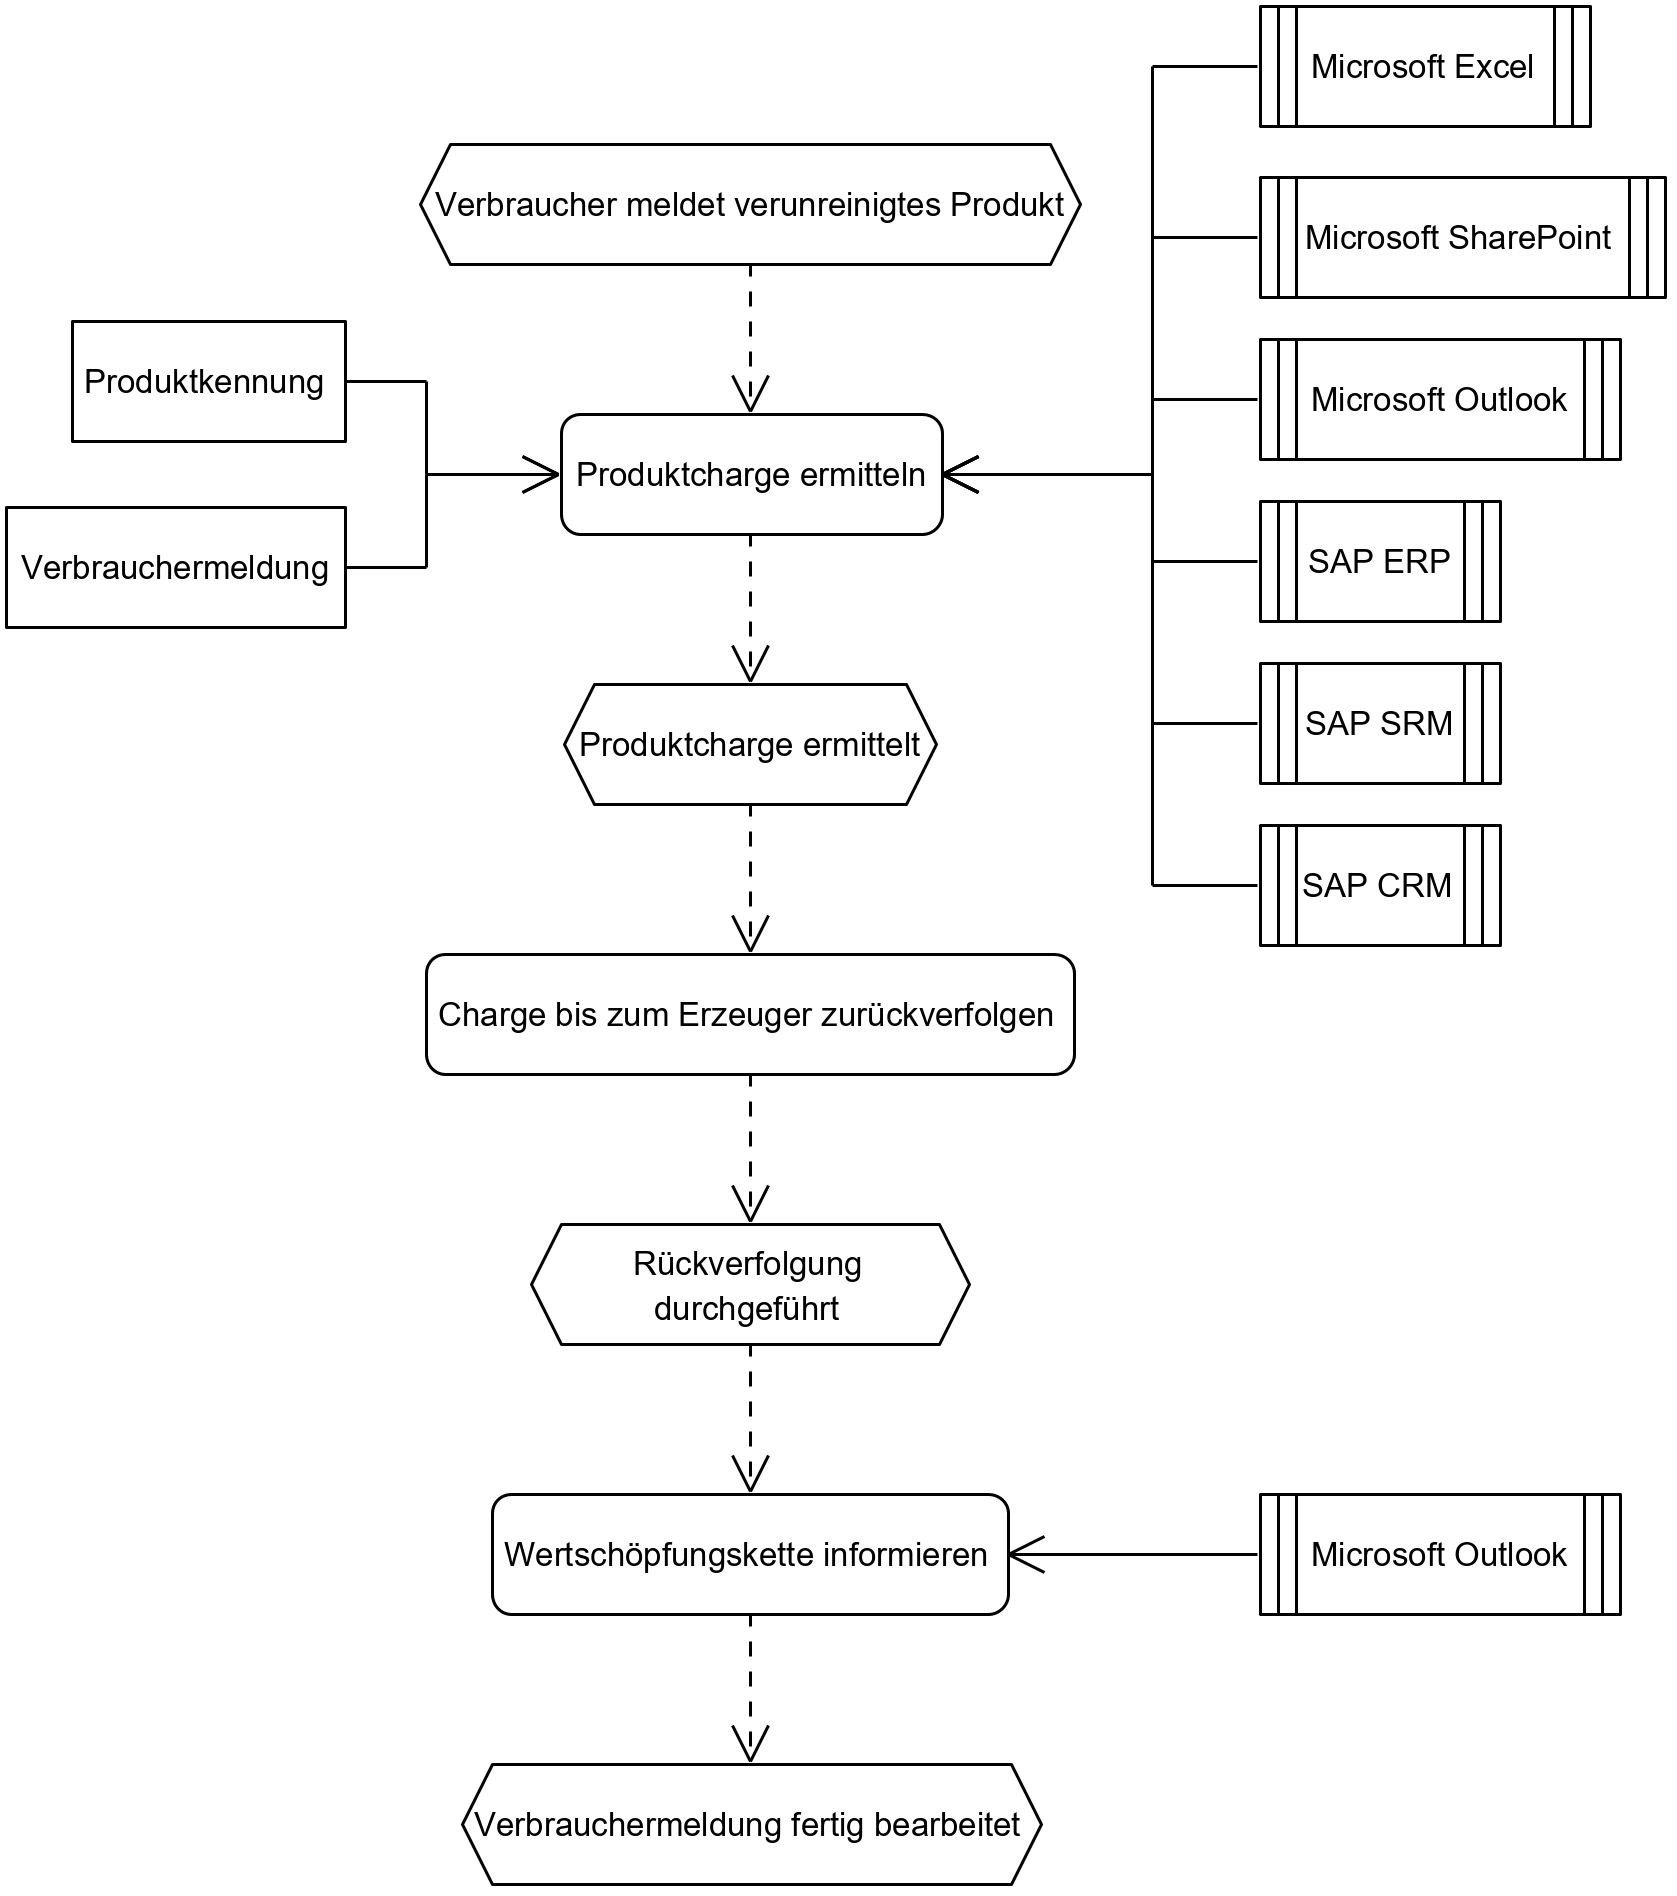
\includegraphics[width=1\linewidth]{pictures/business-process-epc-diagram-bw}
	\caption[Darstellung des Geschäftsprozess Chargenrückverfolgung in eEPK Notation]{Darstellung des Geschäftsprozess Chargenrückverfolgung in eEPK Notation}
	\label{fig:business-process-epc-diagramm}
\end{figure}

\paragraph{Soll-Prozess}
Während im Ist-Prozess (Abbildung \ref{fig:business-process-epc-diagramm}) viele verschiedene IT-Systeme zum Einsatz kommen um alle Chargeninformationen zusammenzutragen, wird im Soll-Prozess das Blockchain Netzwerk und darauf aufsetzende dezentrale Applikationen genutzt. Betrachtet man die einzelnen Prozessschritte so ändert sich bei dem Einsatz einer Blockchain oberflächlich nichts, bei näherer Betrachtung wird dann allerdings deutlich, dass sämtliche Informationen zur Rückverfolgung der Charge vom Blockchain Netzwerk zur Verfügung gestellt werden und nicht in einzelnen Datensilos liegen wie im Ist-Prozess. So dient die Blockchain als gemeinsame Datenbasis für sämtliche Informationen die während der Produktion vom Erzeuger bis zum Lebensmitteleinzelhandel erhoben werden. Änderungen werden transparent in der Blockchain erfasst und sind durch den Konsensmechanismus vor nachträglicher Manipulation geschützt. 

\begin{figure}[H]
	\centering
	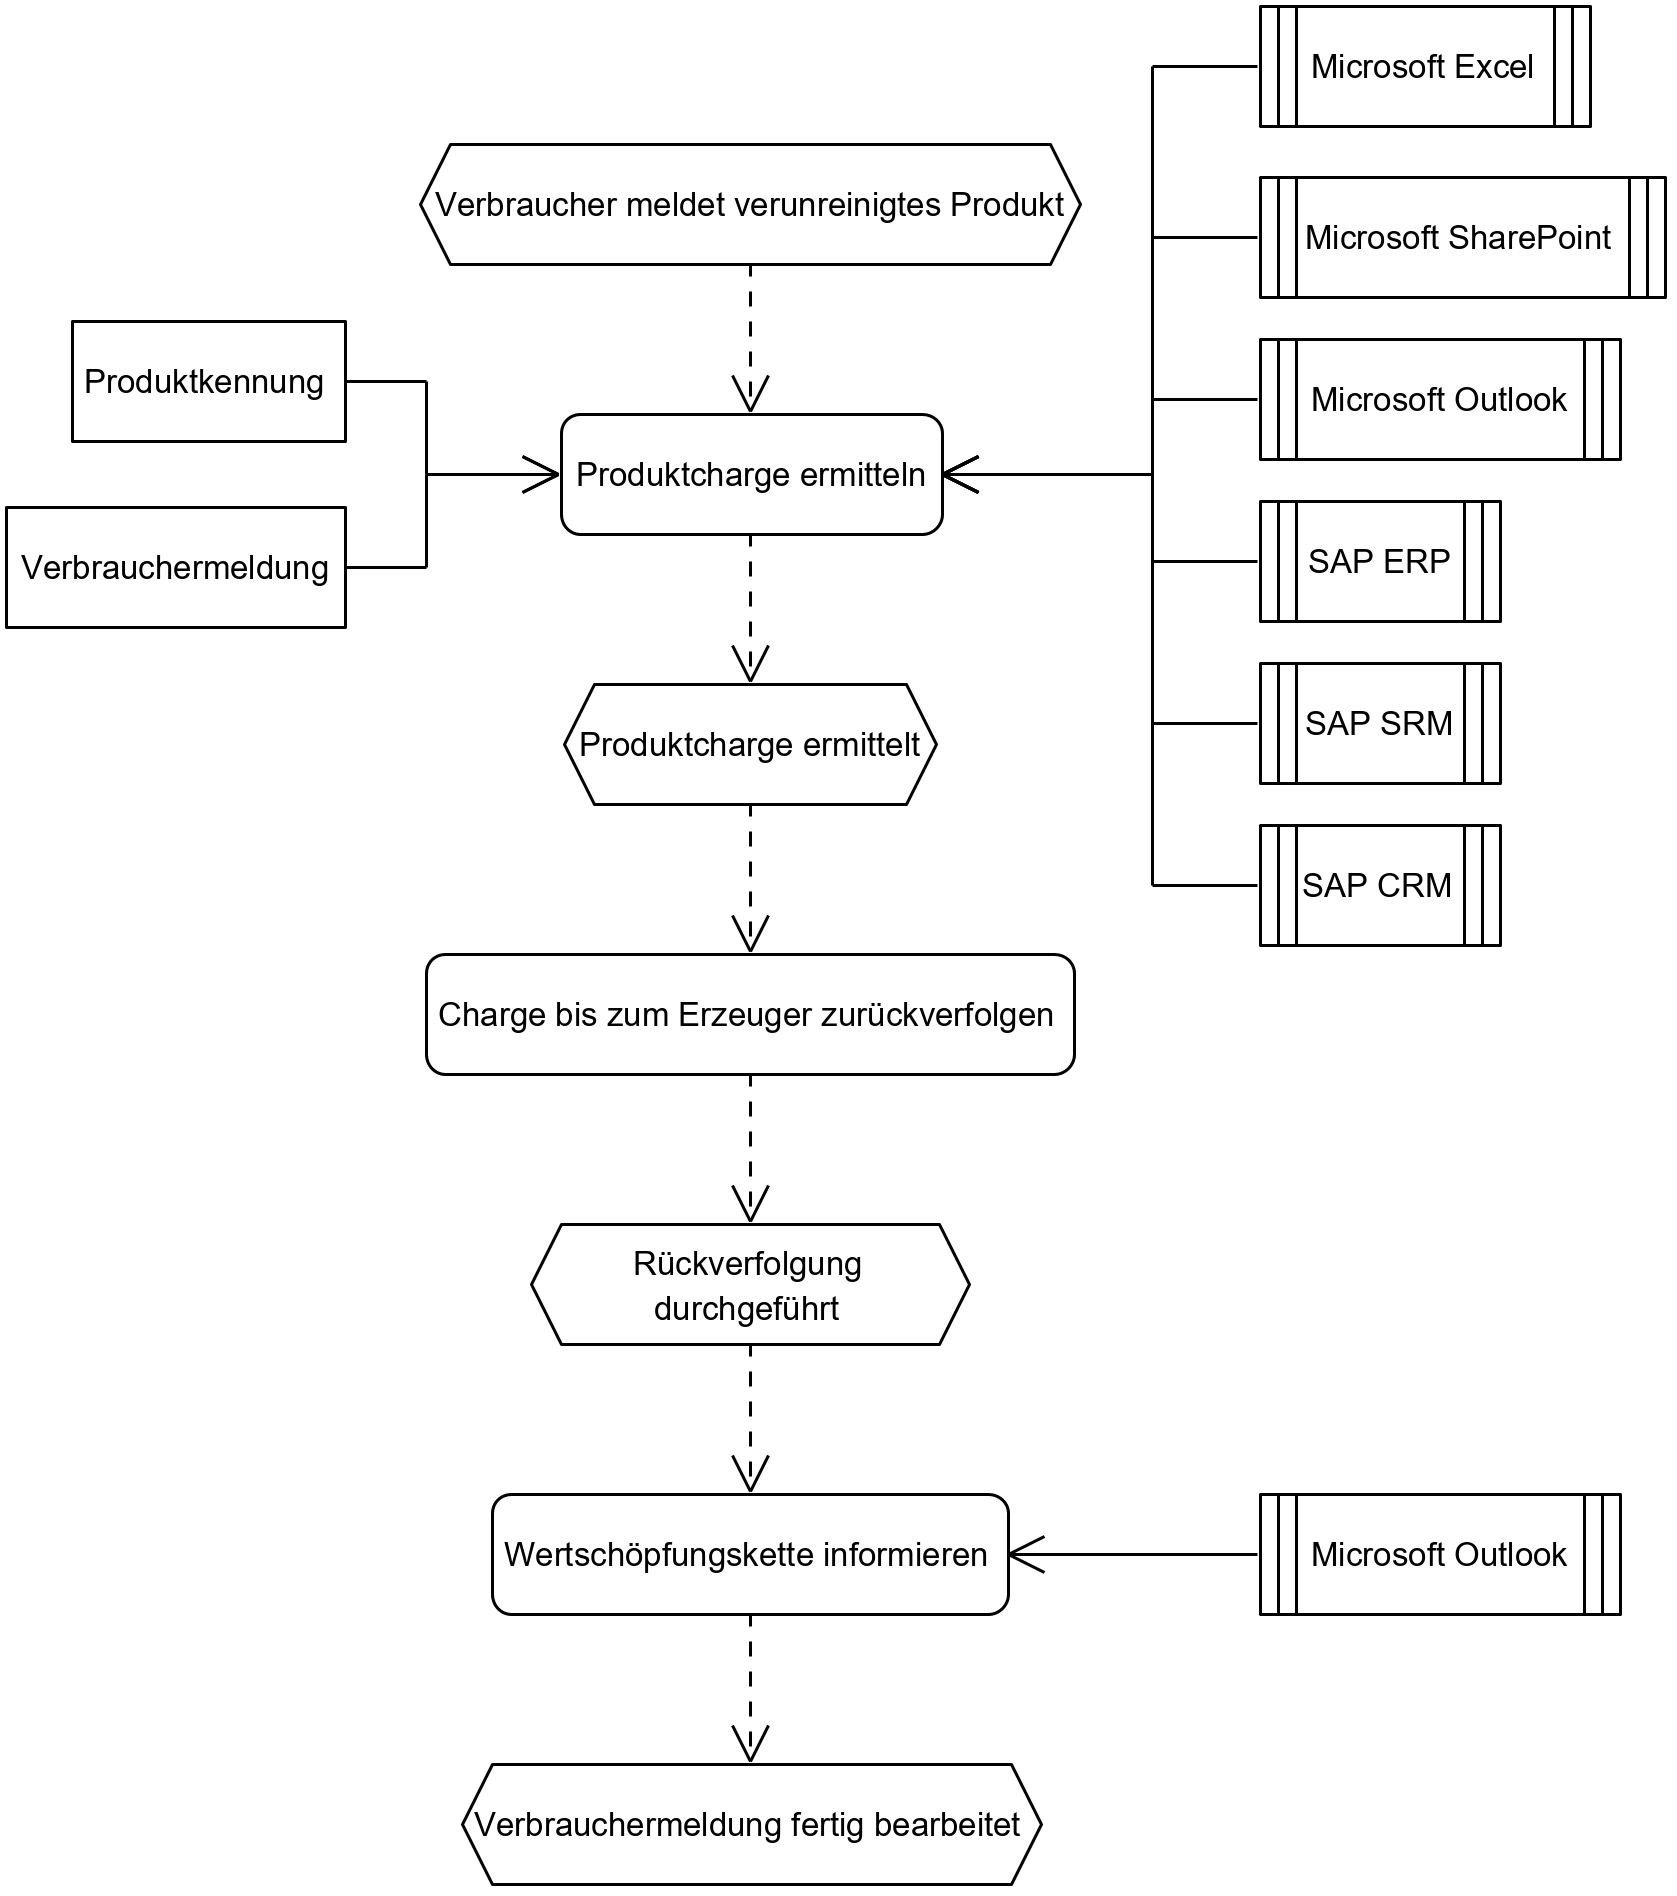
\includegraphics[width=1\linewidth]{pictures/business-process-epc-diagram-bw}
	\caption[Darstellung des Geschäftsprozess Chargenrückverfolgung in eEPK Notation]{Darstellung des Geschäftsprozess Chargenrückverfolgung in eEPK Notation \textcolor{red}{Zu SOLL anpassen}}
	\label{fig:target-business-process}
\end{figure}

\subsection{Systementwurf gemäß Architekturkonzept}\label{system-design-concept}
Unter berücksichtigung der Resultate aus Kapitel \ref{solution-concept} im Kontext des Anwendungsfalls ergibt sich die Grobarchitektur für das System wie in Abbildung \ref{fig:blockchain-system-architecture} dargestellt.

\begin{figure}[H]
	\centering
	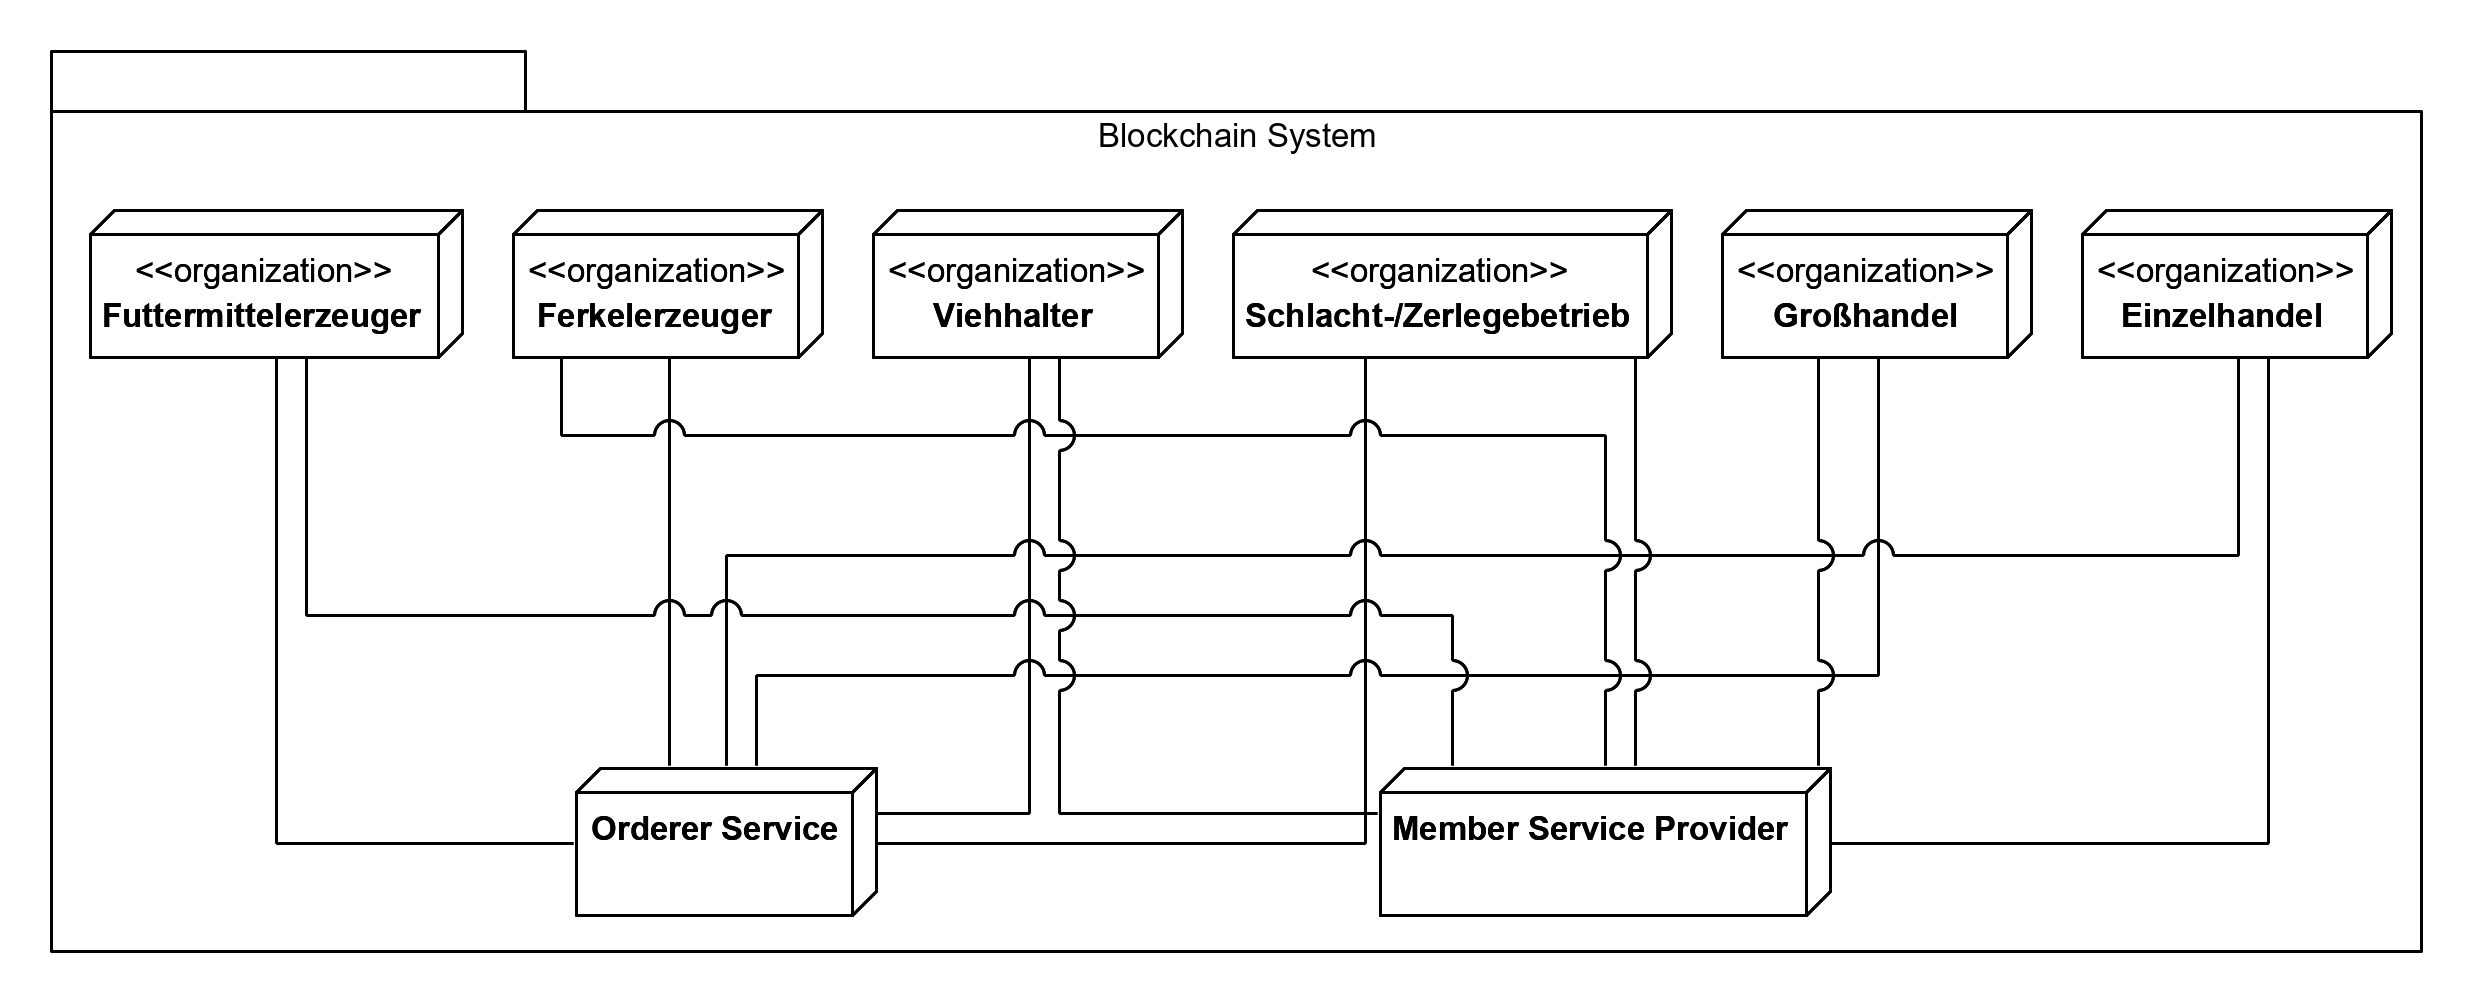
\includegraphics[width=1\linewidth]{pictures/blockchain-system-deployment-diagram}
	\caption[Blockchain System Architektur]{Blockchain System Architektur}
	\label{fig:blockchain-system-architecture}
\end{figure}

Abbildung \ref{fig:organization-component-diagram} zeigt einen Knoten vom Typ \textit{Organization} im Detail. Dem nach besteht eine \textit{Organization} aus logischer Sicht aus dem \textit{Ledger}, einer \textit{Zustandsdatenbank}, den \textit{Smart Contracts} (Chaincode), dem \textit{Konsensmechanismus}, den einzelnen \textit{Teilnehmern} und dem \textit{User Interface}. \textit{Ledger}, \textit{Zustandsdatenbank} und \textit{Smart Contracts} werden zusammen als \textit{Peer} bezeichnet. Wobei die Ausführung der Smart Contracts in einer isolierten Umgebung erfolgt. Zusätzlich gibt es noch eine Sicherheitsstrategie (\ac{ca}) zum Schutz der einzelnen Komponenten. Jeder Teilnehmer des Systems muss mindestens einen \textit{Peer} betreiben, um Transaktionen im Netzwerk erstellen und validieren zu können. Mit jedem zusätzlichen Peer wird die individuelle Ausfallsicherheit der \textit{Organization} erhöht. Nachfolgend werden die einzelnen Komponenten näher beschrieben.

\begin{figure}[H]
	\centering
	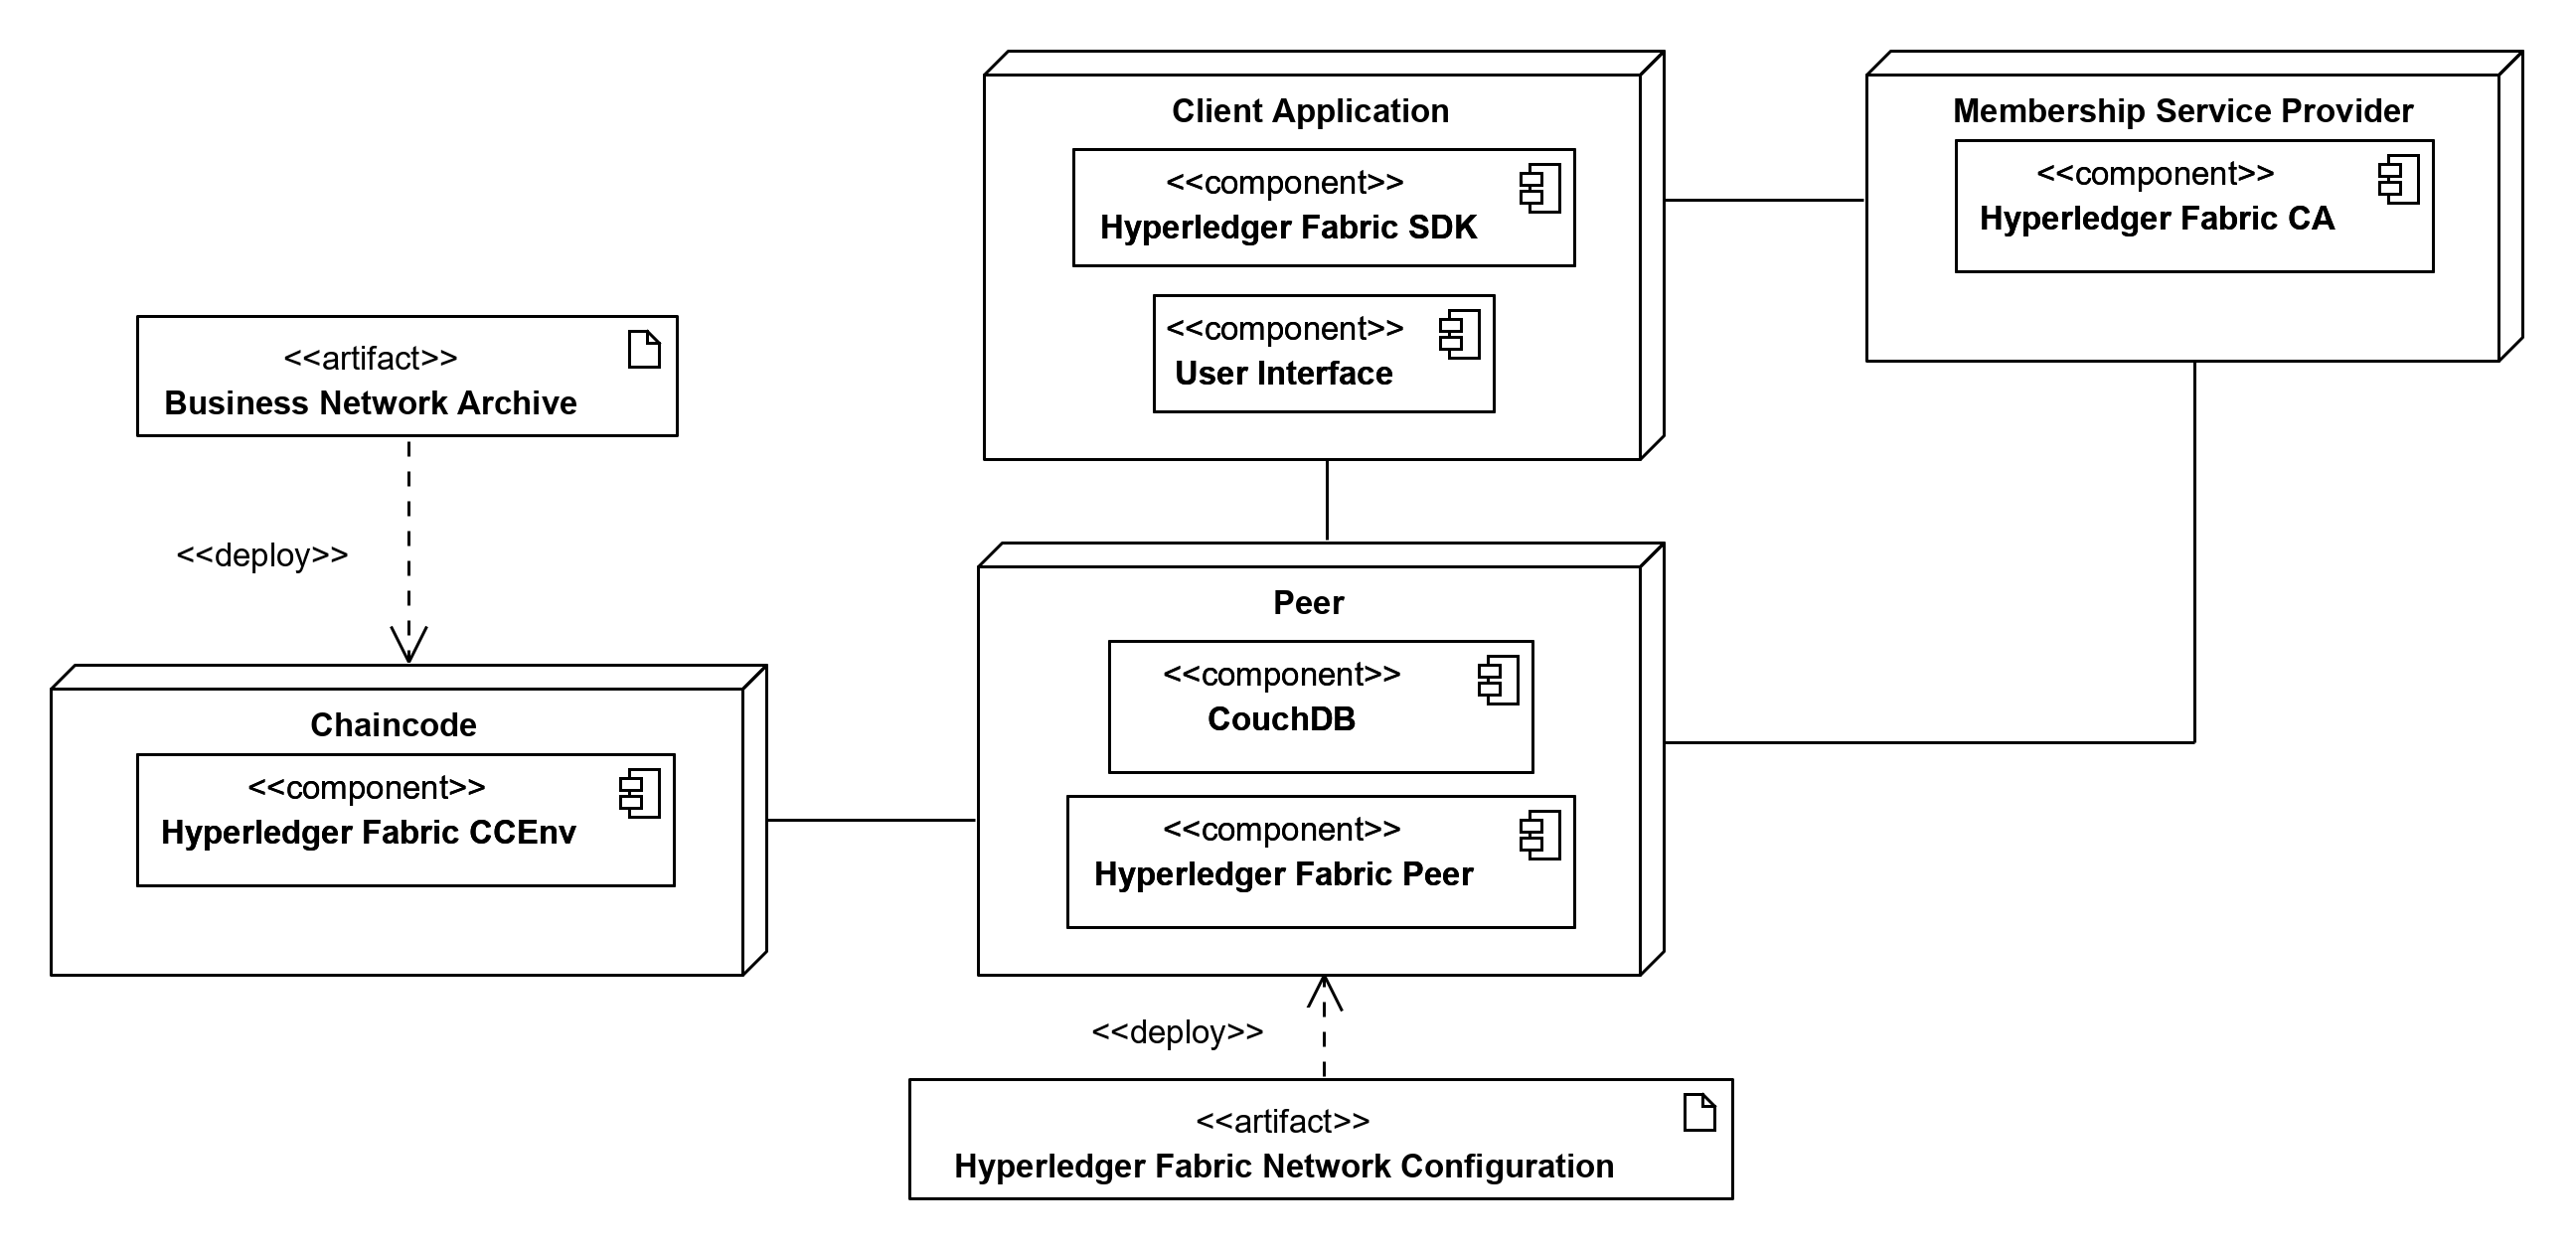
\includegraphics[width=1\linewidth]{pictures/organization-component-diagram}
	\caption[Organisation Komponenten Diagramm]{Organisation Komponenten Diagramm}
	\label{fig:organization-component-diagram}
\end{figure}

\subsubsection{Ledger/Konsens}
Das sogenannte Ledger besteht aus der verketteten Liste der Transaktionen (Hyperledger Fabric Peer), einer Zustandsdatenbank (CouchDB) und dem Orderer Service. Zustandsveränderungen sind Veränderungen aufgrund von Smart Contract Ausführungen, welche durch Teilnehmer oder Smart Contracts ausgelöst werden. Jede Transaktion beschreibt eine Menge von Schlüsselwertpaaren zugehörig zu einem Asset. Assets und die darauf aufbauende Business Netzwerk Definition wird in Kapitel \ref{smart-contracts} näher erläutert. Damit ein Teilnehmer sich gegenüber dem Ledger authentifizieren kann verwendet das Hyperledger Fabric Framework eine \acf{pki}. Diese \ac{pki} wird realisiert durch einen \ac{msp} genannten Service. Dieser Service kümmert sich um die Vergabe und den Abgleich von digitalen Identitäten mit denen sich User gegenüber dem Ledger authentifizieren können. Durch diese Designentscheidung wird das Blockchain Netzwerk ein private permissioned Netzwerk und realisiert damit Anforderung \textit{A2.4}. Eine Anonymität der Teilnehmer ist innerhalb der Lieferkette ohnehin kaum gegeben und nur indirekt über mehrere Produktionsschritte erreichbar. Ein Ziel des Systems ist es transparenz für die Nutzer des Netzwerks zu bieten, aus diesem Grund wurde der Aspekt Anonymität außer acht gelassen. 

Neue Transaktionen im Netzwerk werden über ein User Interface durch einen Teilnehmer ausgelöst. Jede Transaktion durchläuft dann einen dreistufigen Prozess bis sie schlussendlich dem Ledger hinzugefügt wird (Abbildung \ref{fig:transaction-flow}). Die einzelnen Stufen sind 

\begin{itemize}
	\item Endorsement,
	\item Ordering,
	\item Validation.
\end{itemize}

Das Endorsement beginnt mit der Übermittlung der Transaktion zu einem Peer. Dieser verteilt die Transaktion im Netzwerk. Jeder Peer simuliert und prüft nun die Transaktion anhand der Geschäftslogik (Smart Contract). Nach erfolgreicher Prüfung erhält der Transaktionssteller eine Endorsement Signatur, welche an den Orderer Service weitergeleitet wird (Ordering). An dieser Stelle wird die Konsensmechanik durchlaufen und wenn ein Konsens über das Ergebnis der Transaktion hergestellt wurde (Validation) gibt der Orderer Service die Transaktion für das Ledger frei.

\begin{figure}[H]
	\centering
	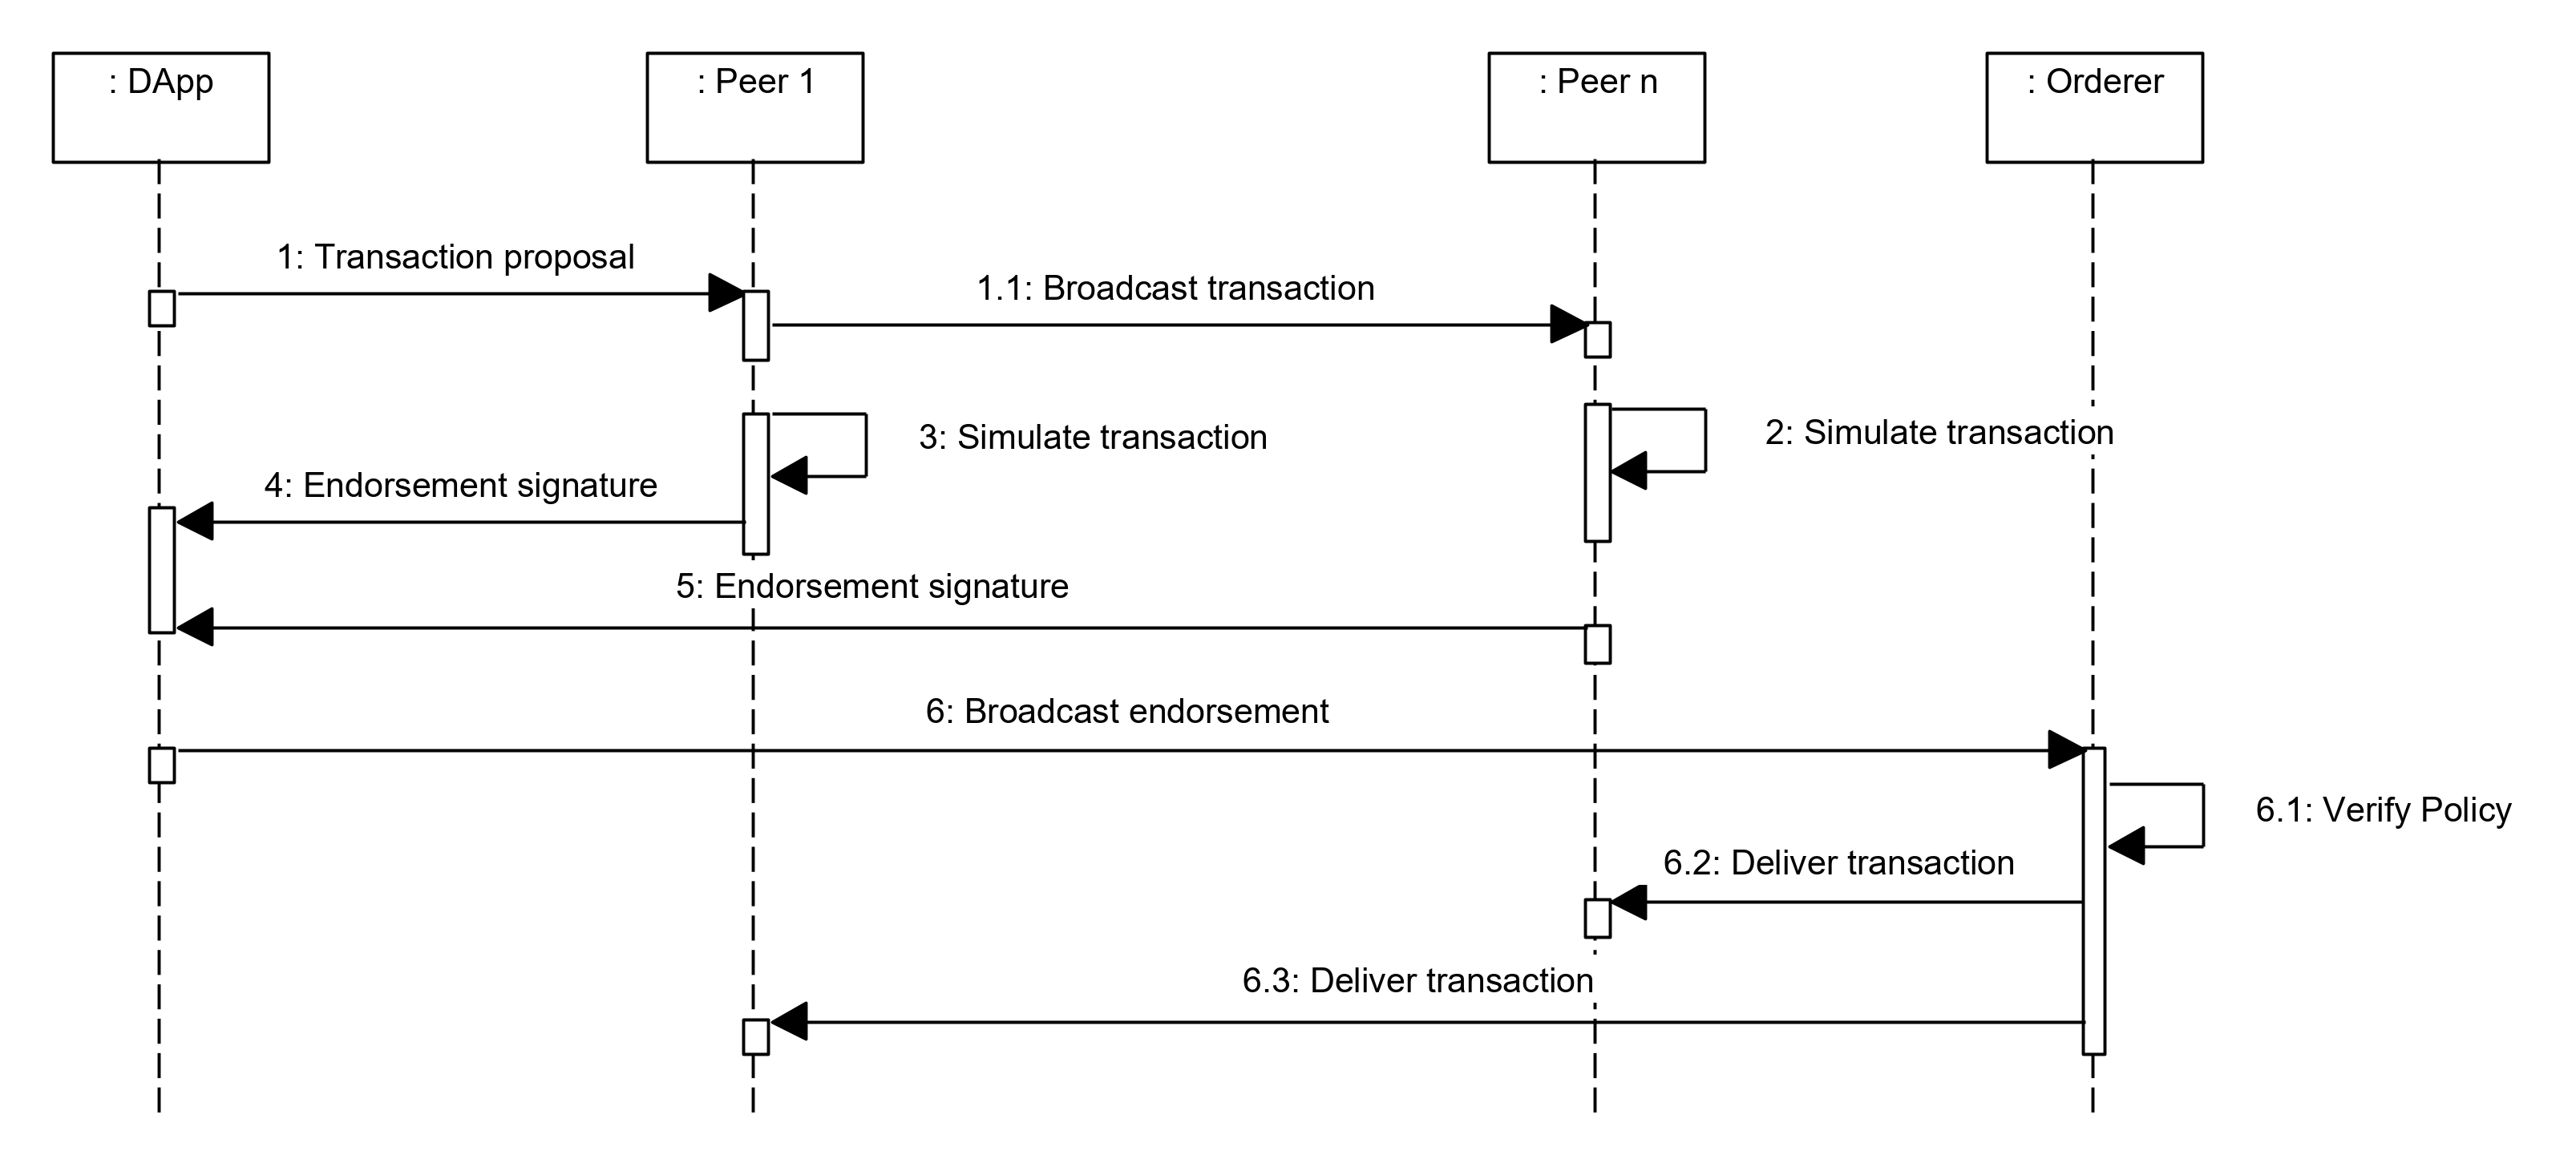
\includegraphics[width=1\linewidth]{pictures/transaction-flow}
	\caption[Transaction Flow]{Transaction Flow in Anlehnung an \citep{Choudhury2018}}
	\label{fig:transaction-flow}
\end{figure}

\subsubsection{Smart Contracts / Business Netzwerk Modell}\label{smart-contracts}
Smart Contracts sind abgebildet als \textit{Transaction Processor Functions}. Zusätzlich werden für Hyperledger Fabric noch Definitionen zu \textit{Participants}, \textit{Assets} und \textit{Queries} erfasst. Diese Komponenten bilden zusammen das \textit{\ac{bna}} und stellen die Geschäftslogik dar. Anforderung \textit{A1.1} wird mit dem \textit{Business Network Archive} realisiert. Hyperledger Fabric bringt eine eigene Modellierungssprache mit. Mit dieser Sprache werden \textit{Assets}, \textit{Participants} und \textit{Transactions} modelliert. Die Sprache unterstützt Vererbung, Templates und abstrakte Klassen, ähnlich der objektorientierten Programmierung.

Damit Transaktionen im Netzwerk verarbeitet werden können, müssen zugehörige \textit{Assets} modelliert und später im System angelegt werden. Für die transparente, lückenlose Rückverfolgung von Chargen sind folgende \textit{Assets} modelliert worden:

\begin{itemize}
	\item \textit{Material}
	\item \textit{Batch}
	\item \textit{BatchNetwork}
\end{itemize}

Mit einem \textit{Asset} \textit{Material} werden die Tiere bzw. Erzeugnisse der Produktionsbetriebe abgebildet. Sie werden identifiziert über eine global eindeutige Nummer. Eine Charge ist definiert als \textit{Batch} und ebenfalls wie ein \textit{Material} global eindeutig identifizierbar. Zur darstellung eines Chargengraphs dient die Entität \textit{BatchNetwork}. Darüber hinaus werden noch \textit{Enumerations} und \textit{Concepts} verwendet, um das modellierte System möglichst modular halten zu können. So ist eine nachträgliche Erweiterung bzw. Anpassung ohne großen Aufwand realisierbar. Es wurden folgende Enumerations und Concepts modelliert:

\begin{itemize}
	\item \textit{MaterialType}
	\item \textit{MaterialQuality}
	\item \textit{TransportLog}
	\item \textit{Location}
	\item \textit{SensorData}
	\item \textit{Status}
\end{itemize}

\begin{figure}[H]
	\centering
	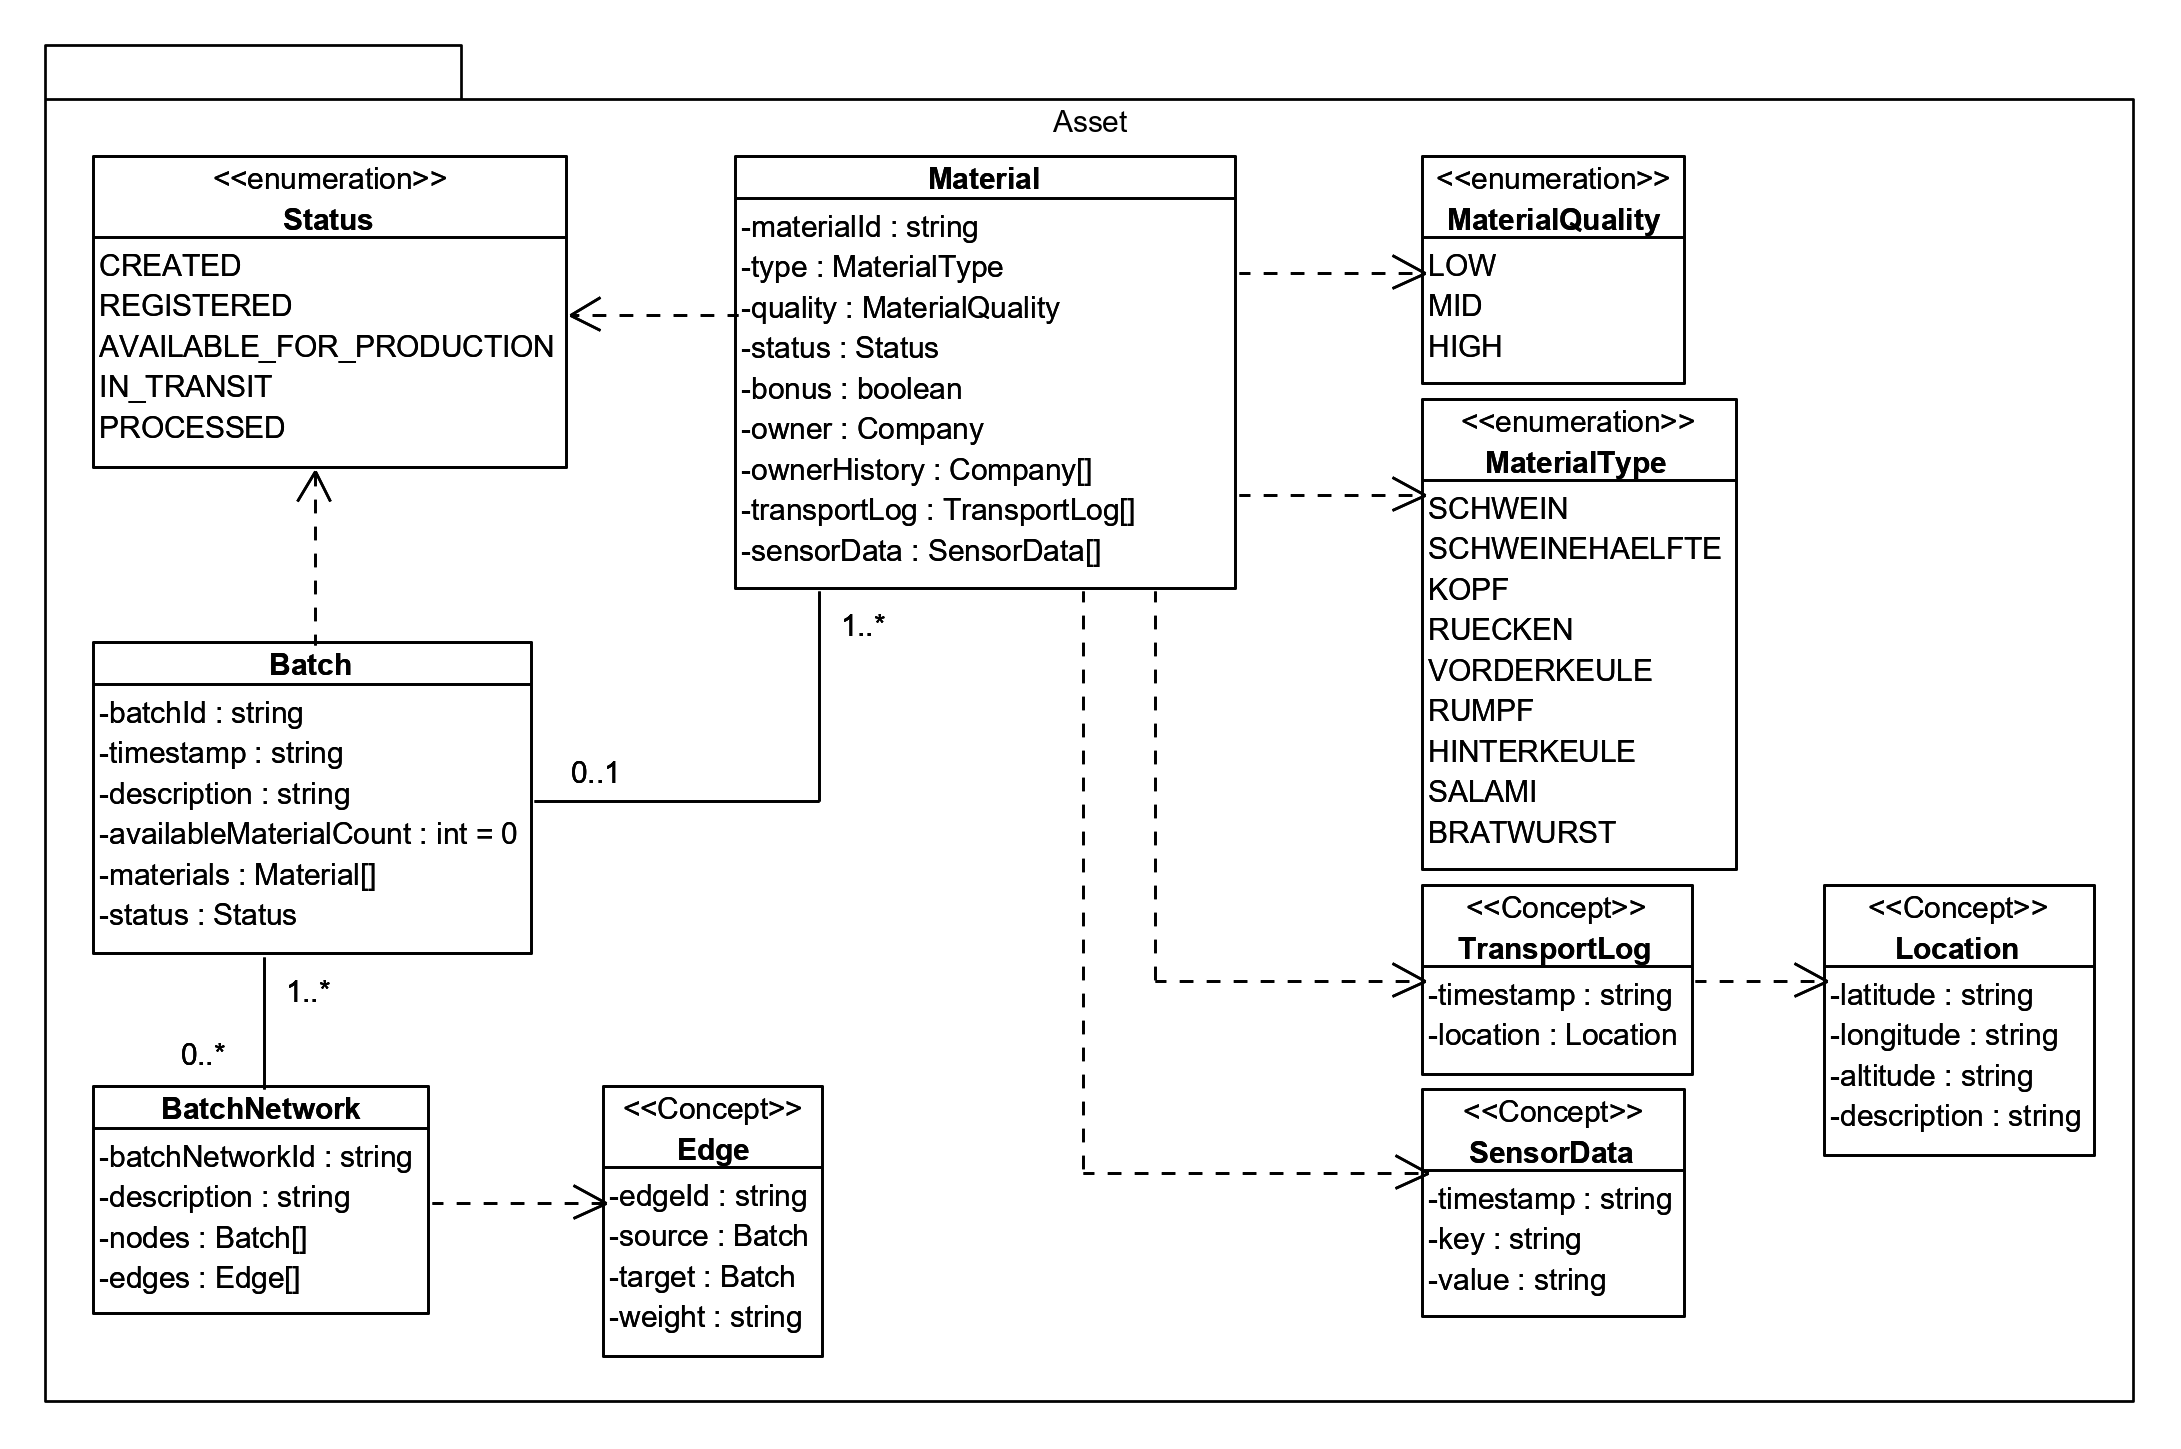
\includegraphics[width=1\linewidth]{pictures/hlc-food-chain-model-assets}
	\caption[Klassendiagramm Blockchain Netzwerk \textit{Assets}]{Klassendiagramm Blockchain Netzwerk \textit{Assets}}
	\label{fig:hlc-food-chain-model-assets}
\end{figure}

Abbildung \ref{fig:hlc-food-chain-model-assets} stellt die Beziehungen zwischen den \textit{Assets}, \textit{Enumerations} und \textit{Concepts} in Form eines UML Klassendiagramms dar.

Die Modellierung der \textit{Participants} ist relativ simpel gehalten. Es gibt eine abstrakte Entität \textit{Company} von der sich jeweils eine Teilnehmerkategorie des Blockchain Netzwerk spezialisiert. Eine \textit{Company} wird identifiziert durch die \ac{gln}\footnote{Die \ac{gln} ist eine zentral vergebene Identifikationsnummer von der GS1-Organisation zur eindeutigen Identifikation von Betriebsstätten.}. Außerdem wurde noch ein komplexer Datentyp in Form eines \textit{Concepts} verwendet. Mit dem \textit{Address} \textit{Concept} wird eine reguläre Geschäftsadresse des Unternehmens abgebildet und als eigenes Attribut der \textit{Company} Entität verwendet. Anforderung \textit{A2.2} wird mit dieser Datenstruktur erfüllt. In Abbildung \ref{fig:hlc-food-chain-model-participants} wird das beschriebene Konstrukt als Klassendiagramm dargestellt.

\begin{figure}[H]
	\centering
	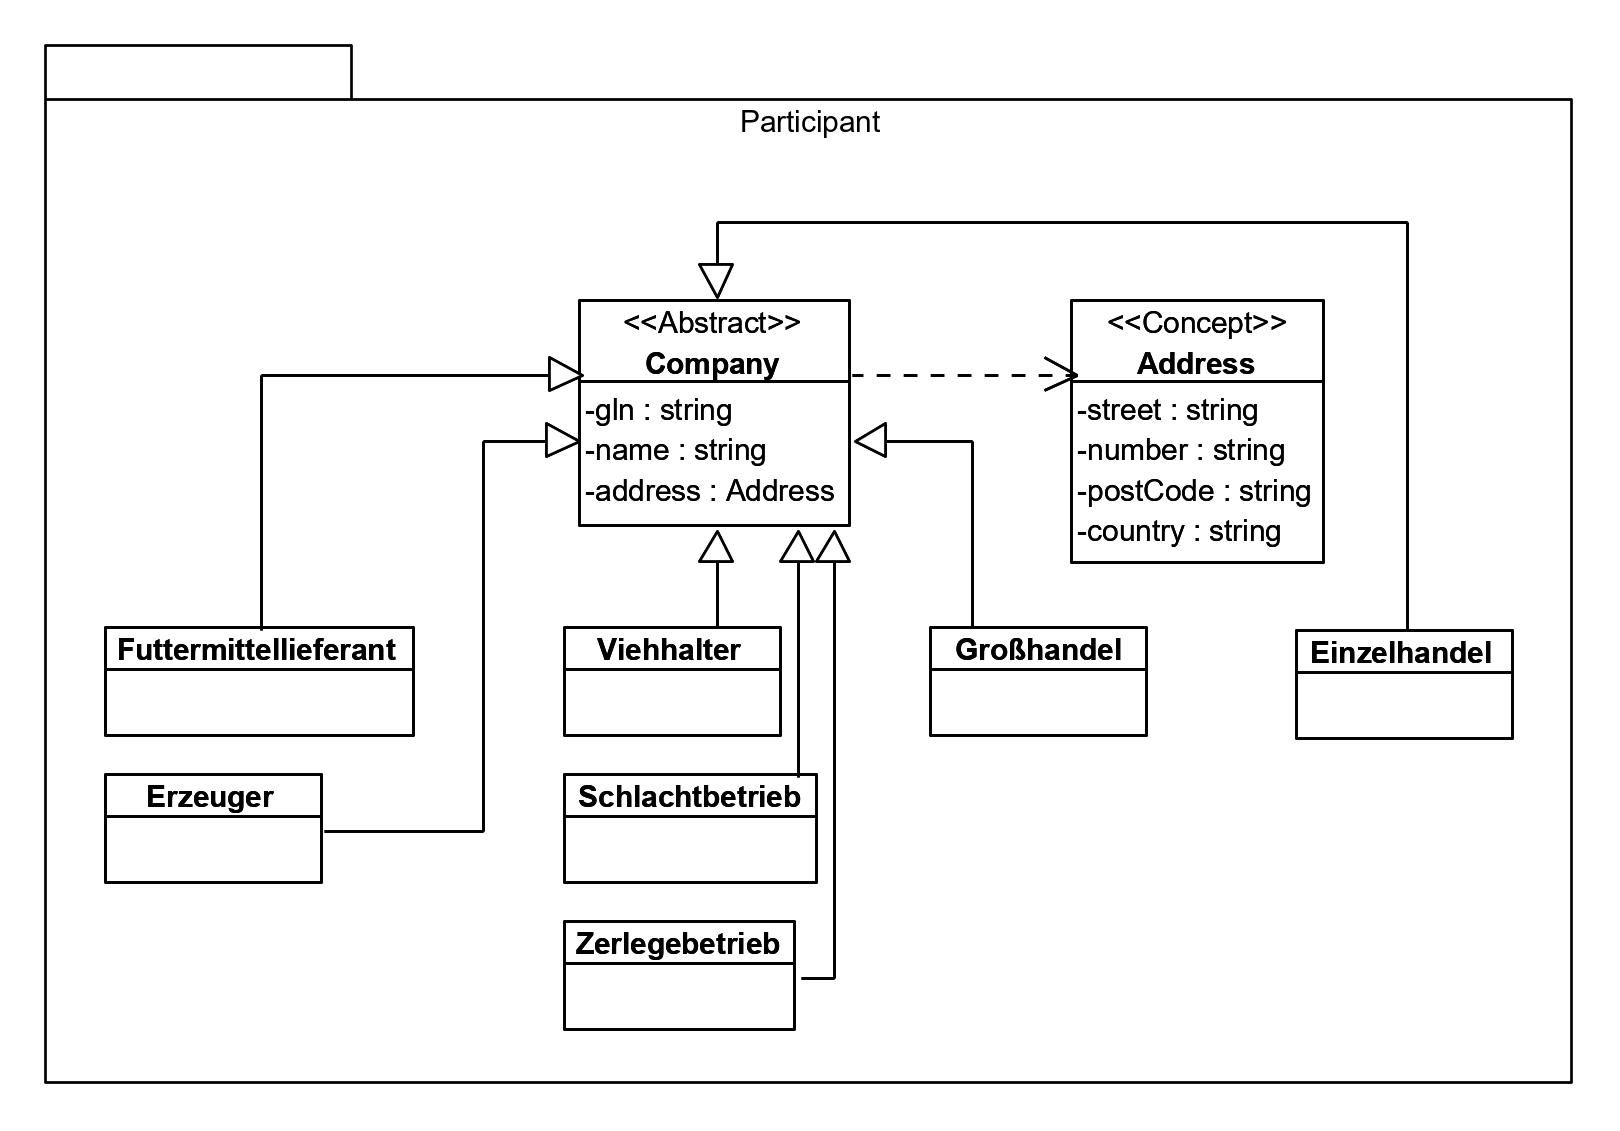
\includegraphics[width=1\linewidth]{pictures/hlc-food-chain-model-participants}
	\caption[Klassendiagramm Blockchain Netzwerk \textit{Participants}]{Klassendiagramm Blockchain Netzwerk \textit{Participants}}
	\label{fig:hlc-food-chain-model-participants}
\end{figure}

Die dritte Komponente des \textit{\ac{bna}} ist die Menge an \textit{Transactions} (Abbildung \ref{fig:hlc-food-chain-model-transactions}). \textit{Transactions} werden von \textit{Participants} ausgelöst und sie verändern oder erzeugen \textit{Assets}. Entsprechend wurden die Geschäftsvorgänge abgebildet die nötig sind um eine Chargenrückverfolgung zu ermöglichen (siehe Kapitel \ref{goal-description}). Es wurde eine \textit{Transaction} modelliert zum erzeugen von neuem Material - \textit{produceMaterial}. Diese \textit{Transaction} verlangt mehrere Parameter. Bis auf den Parameter \textit{newMaterial} sind alle weiteren Parameter optional. \textit{newMaterial} enthält alle Daten für ein neues Tier, das im Netzwerk registriert wird. Die optionalen Parameter werden verwendet, wenn in späteren Produktionsschritten vorhandene Erzeugnisse zu Zwischenprodukten weiterverarbeitet werden. Des weiteren sind \textit{Transactions} modelliert mit denen die Eigentumsverhältnisse eines \textit{Assets} verändert werden können. Außerdem lassen sich Chargen angelegen und mit registrierten Tieren verknüpfen. 

\begin{figure}[H]
	\centering
	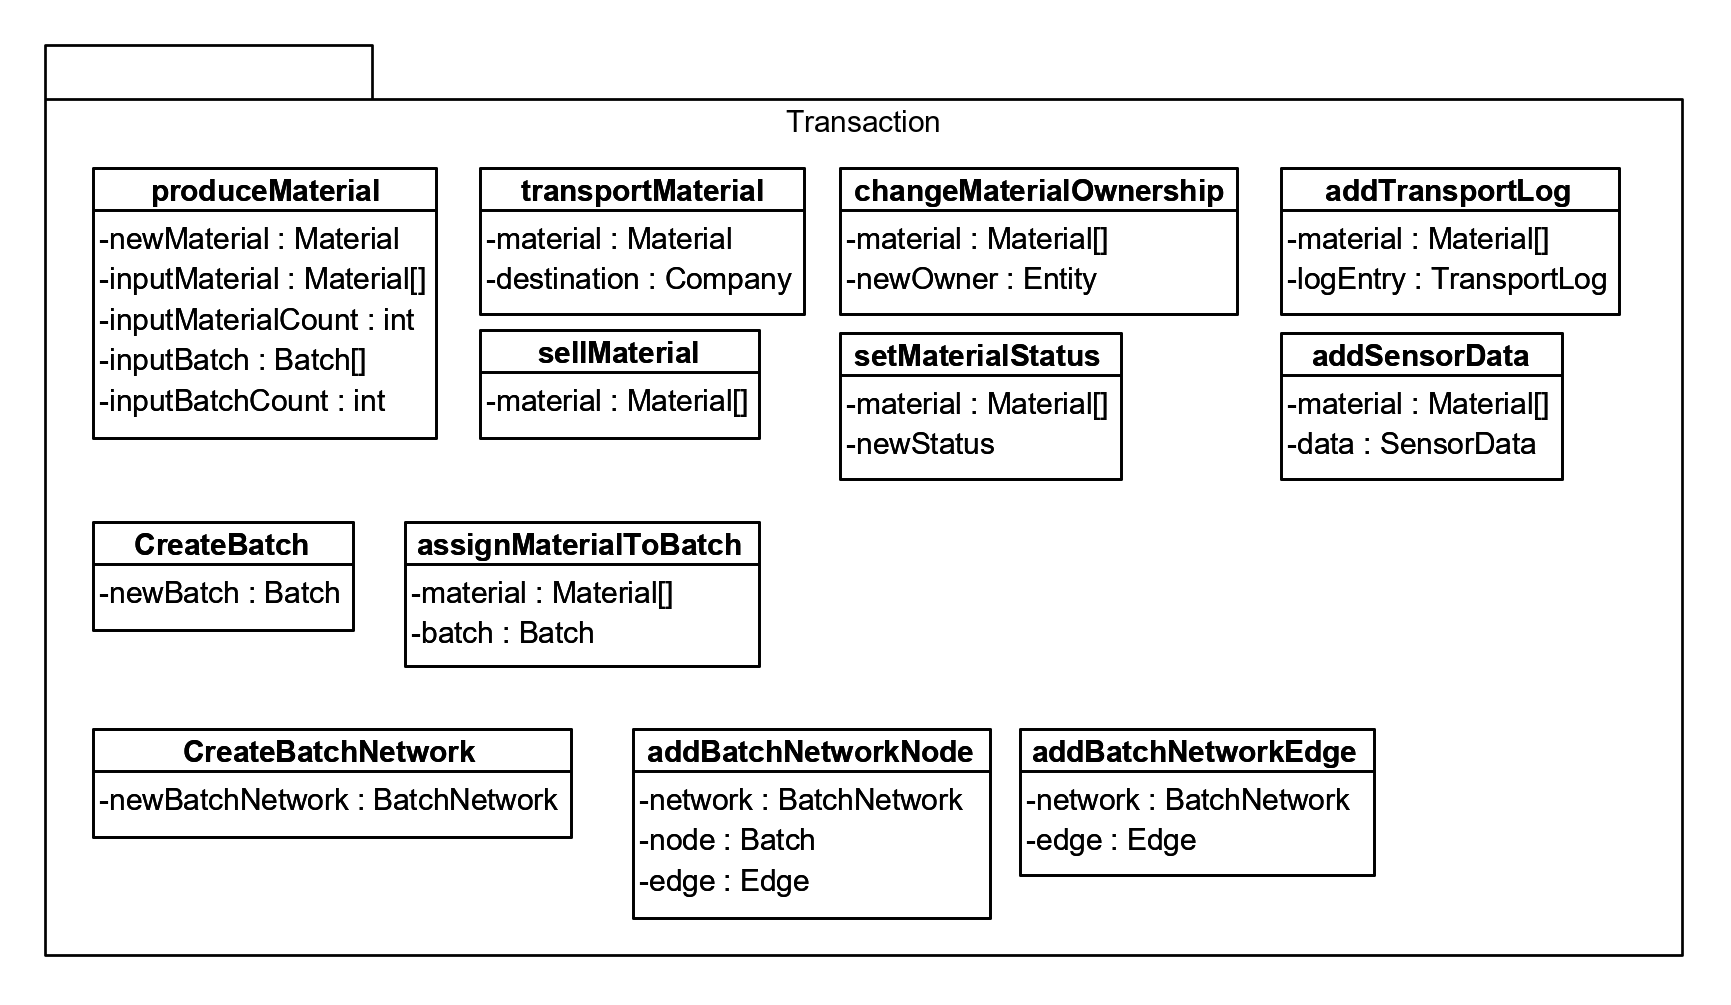
\includegraphics[width=1\linewidth]{pictures/hlc-food-chain-model-transactions}
	\caption[Klassendiagramm Blockchain Netzwerk \textit{Transactions}]{Klassendiagramm Blockchain Netzwerk \textit{Transactions}}
	\label{fig:hlc-food-chain-model-transactions}
\end{figure}

% \subsubsection{API (REST)}
% Endpoint Beschreibung\\
% 3.1 REST API

\subsubsection{Identity Management}
Administration und Interaktion mit dem System wird über ein Identity Management organisiert. Da es sich bei dem System um ein private permissioned Ledger handelt, sind per Definition (Kapitel \ref{Arten-von-Blockchain}) alle Teilnehmer untereinander vollständig bekannt und es gibt keine Anonymität. Dies wird durch den \textit{Membership Service Provider} realisiert. Die verwendete \acf{pki} besteht dabei aus

\begin{itemize}
	\item einer Registrierungsstelle (RA), die die Identität von Instanzen überprüft, die ihre digitalen Zertifikate in der CA speichern möchten,
	\item einer Zertifizierungsstelle (CA), die die digitalen Zertifikate speichert, ausstellt und signiert,
	\item einem zentralen Verzeichnis, d. h. einer sicheren Datenbank zum Speichern und für das Indexieren von Schlüsseln,
	\item einem Zertifikatsverwaltungssystem, das beispielsweise den Zugriff auf gespeicherte Zertifikate oder die Zustellung der auszugebenden Zertifikate verwaltet,
	\item einer Zertifikatsrichtlinie mit den Anforderungen der \ac{pki} für ihre Verfahren. Außenstehende können damit die Vertrauenswürdigkeit der \ac{pki} analysieren.
\end{itemize}

Am Beispiel der Zertifikatsausstellung soll die Funktionsweise des \textit{Membership Service Providers} dargestellt werden. Zur Veranschaulichung des Ablaufs dient Abbildung \ref{fig:hyperledger-fabric-membership-blockchain}.

\begin{figure}[H]
	\centering
	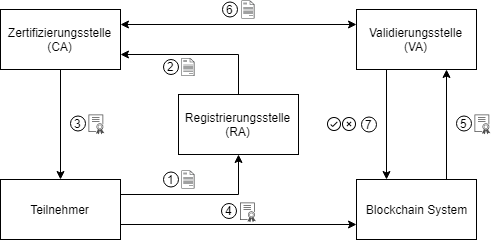
\includegraphics[width=1\linewidth]{pictures/digital-identity-issue}
	\caption[Ausstellen einer digitalen Identität für einen Teilnehmer der Blockchain]{Ausstellen einer digitalen Identität für einen Teilnehmer der Blockchain}
	\label{fig:hyperledger-fabric-membership-blockchain}
\end{figure}

Bevor eine Transaktion ins Netzwerk zur Verarbeitung eingebracht werden kann, muss sich ein Teilnehmer gegenüber dem System authentifizieren. Hierfür ist ein gültige Ausweisdokument (in diesem Beispiel die digitale Identität) notwendig. Um diese ausgehändigt zu bekommen, werden folgende Schritte durchlaufen: Der entsprechende Teilnehmer meldet sich bei der zuständigen Stelle zur Registration (siehe Abbildung: Registrierungsstelle RA) und beantragt ein Ausweisdokument (1). Damit das Ausweisdokument eindeutig zugeordnet werden kann, ist dieses mit den für den Teilnehmer notwendigen und spezifischen Informationen ausgestattet. Die Registrierungsstelle überprüft die hinterlegten Informationen und bestätigt (2) diese gegenüber der Zertifizierungsstelle (CA), welche im nachfolgenden Schritt das entsprechende Zertifikat (digitale Identität) ausstellt (3). Mit Hilfe dieses Zertifikats kann sich der Teilnehmer dann gegenüber dem System authentifizieren (4). Zur Überprüfung der Gültigkeit und Integrität des Dokuments wird die digitale Identität im abschließenden Schritt gegenüber einer Validierungsstelle geprüft (5). Diese gleicht alle hinterlegten Informationen der CA (6) mit dem vorliegenden Dokument ab und bestätigt im Idealfall zum einen die Echtheit der Person und zum anderen auch die Echtheit und den Inhalt des Zertifikats (7). Der Teilnehmer beweist mithilfe der digitalen Identität, dass es sich wirklich um diesen Teilnehmer handelt.

Der \textit{Membership Service Provider} ist so konzipiert, dass er bei Bedarf auch extern bereitgestellt werden könnte. So ist den Teilnehmern freigestellt, ob sie den Dienst selber betreiben oder das gesamte Netzwerk beispielsweise durch eine externe Zertifikatstelle die Identitätsvergabe regelt.

\subsubsection{User Interface / \DH Apps}
Endanwender sollen mit dem Gesamtsystem über GUI-Applikationen interagieren. Dazu wurden Mockups für die einzelnen Oberflächen designt. Der Einstieg erfolgt über eine sogenannte Launchpad Seite. Alle weiteren Applikationen lassen sich vom Launchpad aus erreichen. Das Launchpad dient dem Endanwender als zentrale Anlaufstelle um alle Geschäftsvorgänge abzuwickeln. Applikationen werden als Kachel in unterschiedlichen Gruppen angezeigt. Dabei wurde jeweils eine Gruppe für Asset Operationen und Chargen Operationen modelliert (siehe Abbildung \ref{fig:ui-launchpad}). Die Kacheln sind nach dem Ablauf des Lebenszyklus angeordnet. Beginnend mit der Anmeldung eines neuen Tieres im Netzwerk (\textit{Register Asset}).

\begin{figure}[H]
	\centering
	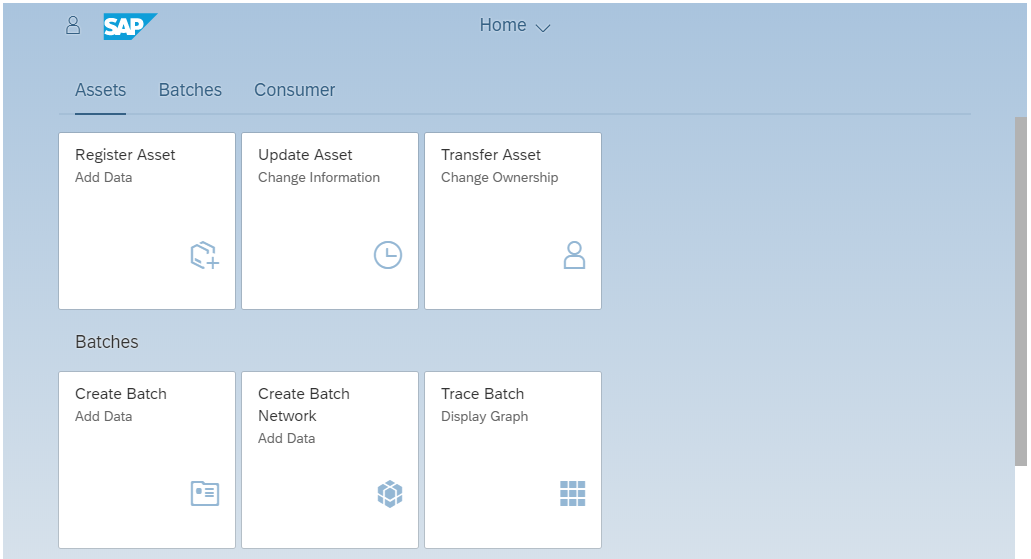
\includegraphics[width=1\linewidth]{pictures/ui-launchpad}
	\caption[Mockup: Einstiegsseite Endanwender]{Mockup: Einstiegsseite Endanwender}
	\label{fig:ui-launchpad}
\end{figure}

Über diese Oberfläche kann ein Anwender die Eigenschaften des zu registrierenden Tieres erfassen. Zwingend nötige Informationen sind mit einem Stern am Beginn der Formularzeile markiert (Abbildung \ref{fig:ui-register-asset}). So sind bei einem Ferkel beispielsweise keine Tiere weiterverarbeitet worden (Formularfeld \textit{Processed Assets}) sondern es stellt den Anfang des Warenstroms dar. Wenn ein Ferkel zum Mastbetriebt transportiert wurde und der Mastbetrieb dann ein schlachtreifes Schwein erfassen will hat er die Möglichkeit das Ferkel bei der Registrierung des Schweins mitanzugeben. Innerhalb der Transaktionslogik kann dann auf diese Information reagiert werden. Im einfachsten Fall erfährt das verarbeitete Asset eine Statusänderung.

\begin{figure}[H]
	\centering
	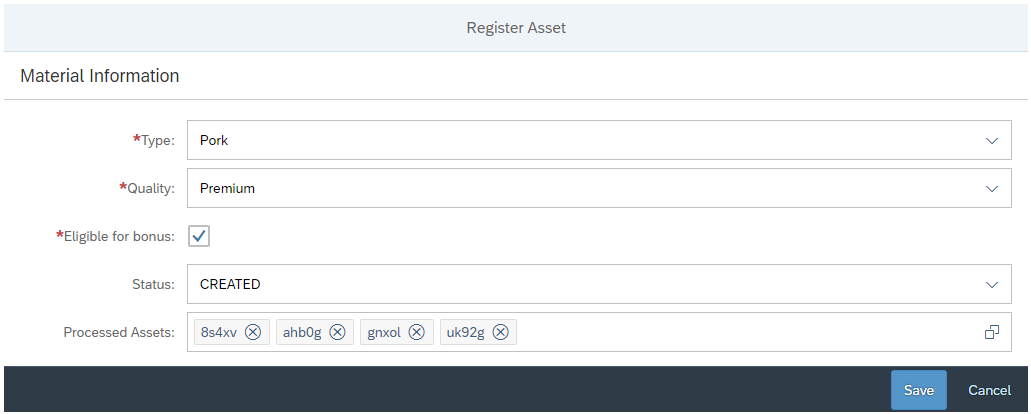
\includegraphics[width=1\linewidth]{pictures/ui-register-asset}
	\caption[Mockup: Asset Registrierung]{Mockup: Asset Registrierung}
	\label{fig:ui-register-asset}
\end{figure}

Des weiteren wurde eine Applikation modelliert mit der bereits erfasste Assets gepflegt werden können. Wie in Abbildung \ref{fig:ui-update-asset} durch die ausgegrauten Eingabefelder dargestellt, können bei einem vorhandenen Asset nicht alle Informationen nachträglich verändert werden. Schlüsselmerkmale wie die Identifikationsnummer werden vom System automatisch generiert beim Erfassen eines Assets und können daher nicht vom Anwender angepasst werden.

\begin{figure}[H]
	\centering
	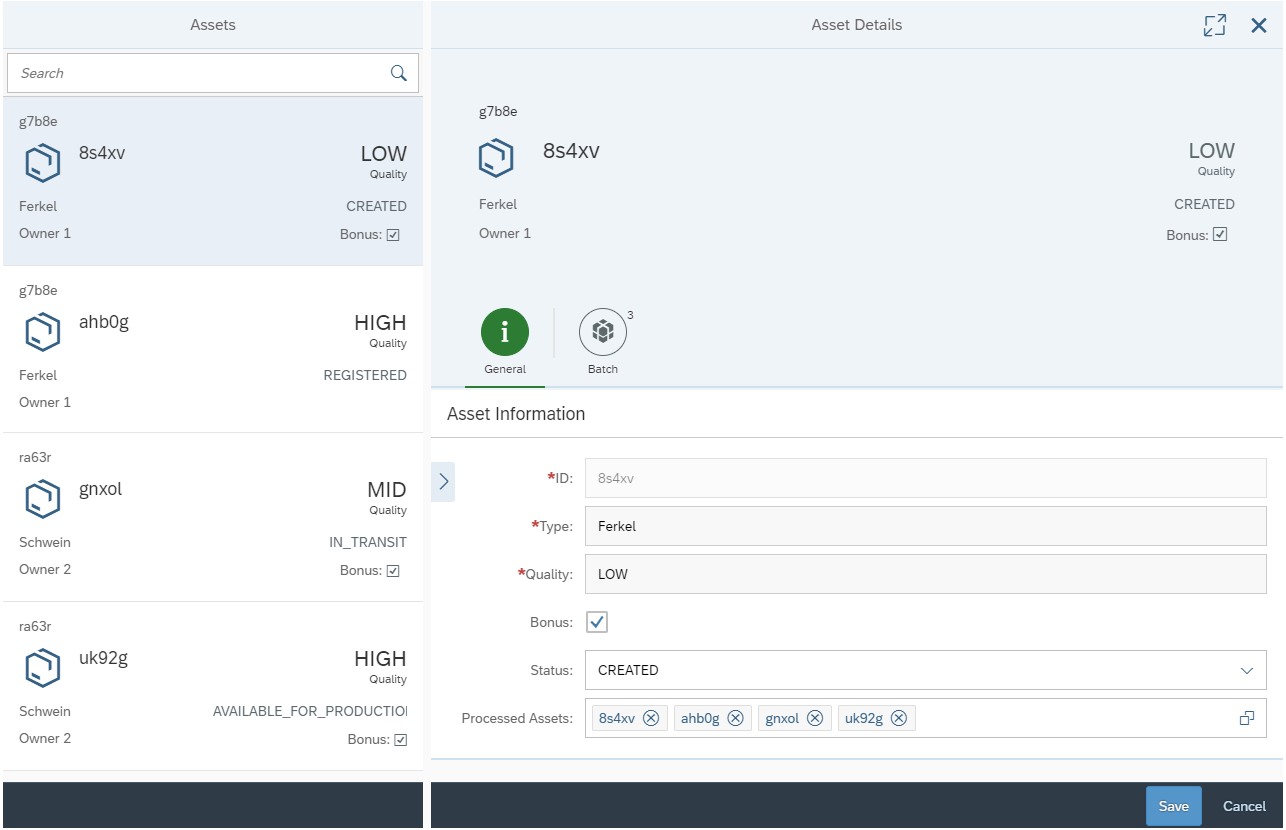
\includegraphics[width=1\linewidth]{pictures/ui-update-asset}
	\caption[Mockup: Asset Update]{Mockup: Asset Update}
	\label{fig:ui-update-asset}
\end{figure}



\begin{figure}[H]
	\centering
	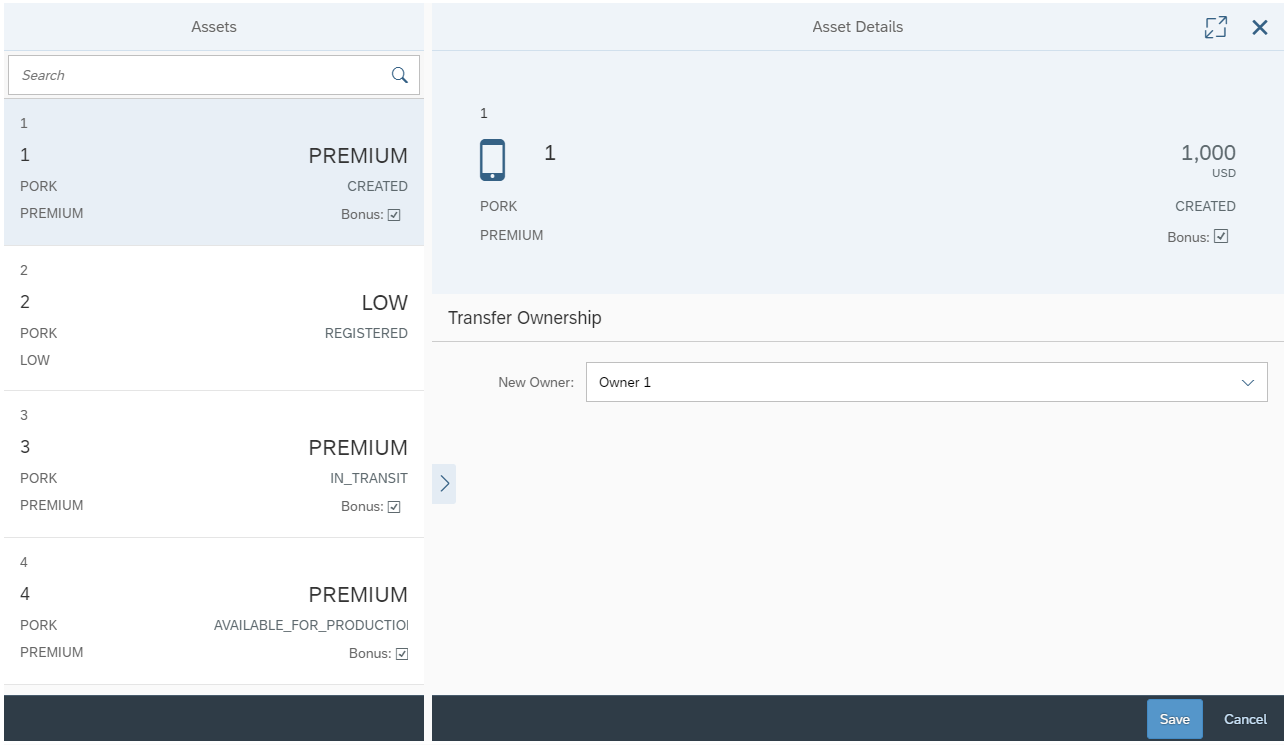
\includegraphics[width=1\linewidth]{pictures/ui-transfer-asset}
	\caption[Mockup: Asset Transfer]{Mockup: Asset Transfer}
	\label{fig:ui-transfer-asset}
\end{figure}

Äquivalent zu den Assets wurden ebenfalls Applikationen zum Anlegen und Pflegen von Chargen modelliert. 

\begin{figure}[H]
	\centering
	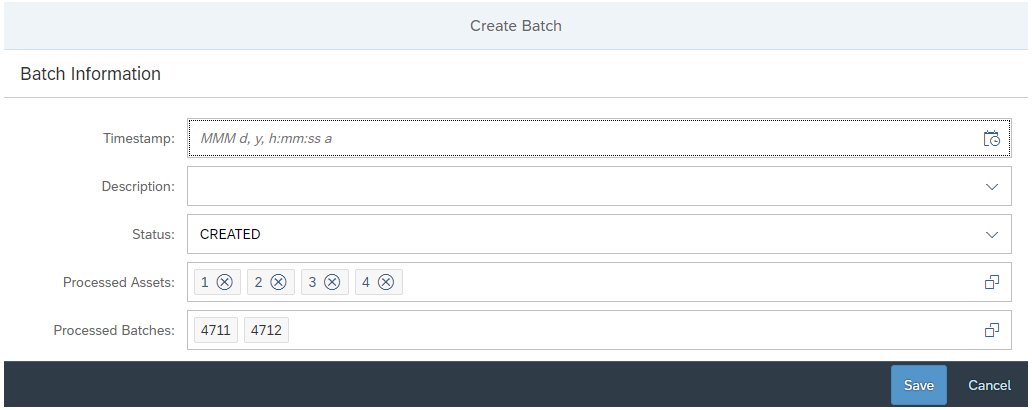
\includegraphics[width=1\linewidth]{pictures/ui-create-batch}
	\caption[Mockup: Batch Create]{Mockup: Batch Create}
	\label{fig:ui-create-batch}
\end{figure}

% Display Batch
% \begin{figure}[H]
% 	\centering
% 	\includegraphics[width=1\linewidth]{pictures/ui-display-batch}
% 	\caption[Mockup: Asset Registrierung]{Mockup: Asset Registrierung}
% 	\label{fig:ui-display-batch}
% \end{figure}

% Display Batch Network
% \begin{figure}[H]
% 	\centering
% 	\includegraphics[width=1\linewidth]{pictures/ui-display-batch-network}
% 	\caption[Mockup: Asset Registrierung]{Mockup: Asset Registrierung}
% 	\label{fig:ui-display-batch-network}
% \end{figure}

% \subsubsection{Security / Permissions / Access-Control-List}
% Permissions.acl Vorgaben\\

\subsection{Zusammenfassung Systementwurf}

Mit dem Kapitel Systementwurf wurde die Methode der Anforderungserhebung beschrieben und eine Zieldefinition gegeben. Daneben sollte eine Betrachtung der Wertschöpfungskette und des Geschäftsprozess in Ist- und Soll-Variante aufzeigen an welchen Punkten ein Blockchain System im Prozess eingesetzt werden sollte um den Gesamtprozess der Chargenrückverfolgung zu unterstützen bzw. überhaupt erst möglich zu machen. Abschließend wurde der Systementwurf beschrieben unterteilt in Ledger/Konsens, Smart Contracts, Identity Management und dem User Interface. Im nächsten Kapitel wird dann die technische Umsetzung des Systementwurf für den Prototyp detailiert beschrieben.

\newpage
